\mfpicnumber{1}

\opengraphsfile{RootRadicalFunctions}

\setcounter{footnote}{0}

\label{RootRadicalFunctions}

\co{In Sections \ref{ConstantandLinearFunctions}, \ref{AbsoluteValueFunctions} and \ref{QuadraticFunctions}, we studied constant, linear,  absolute value,\footnote{These were introduced, as you may recall, as piecewise-defined linear functions.} and quadratic functions.  Constant, linear and quadratic functions were specific examples of polynomial functions, which we studied in generality in Chapter \ref{PolynomialFunctions}. \co{Chapter \ref{PolynomialFunctions} culminated with the Real Factorization Theorem, Theorem \ref{realfactorization}, which says that all polynomial functions with real coefficients can be thought of as products of linear and quadratic functions.}  Our next step was to enlarge our field\footnote{This is a really bad math pun.} of study to rational functions in Chapter \ref{RationalFunctions}.  Being quotients of polynomials, we can ultimately view this family of functions as being built up of linear and quadratic functions as well.  So in some sense, Sections   \ref{ConstantandLinearFunctions}, \ref{AbsoluteValueFunctions} and \ref{QuadraticFunctions} along with Chapters \ref{PolynomialFunctions} and \ref{RationalFunctions} can be thought of as an exhaustive study of linear and quadratic\co{\footnote{If we broaden our concept of functions to allow for complex valued coefficients, the Complex Factorization Theorem, Theorem \ref{complexfactorization}, tells us every function we have studied thus far is a combination of linear functions.}} functions.}  We now turn our attention to functions involving radicals which cannot be written in terms of linear functions.  For a more detailed review of the basics of roots and radicals, we refer the reader to Sections \ref{AppRealNumberArithmetic} and  \ref{AppRadEqus}.  




\subsection{Root Functions}
\label{RootFunctions}

As with polynomial functions and rational functions, we begin our study of functions involving radical with a special family of functions: the (principal) root functions.

\smallskip

\colorbox{ResultColor}{\bbm

\begin{defn}[$n^{th}$ (principal) root function] \label{principalrootfunction}  Let $n \in \mathbb{N}$ with $n \geq 2$.  The \index{$n$th root function}\index{function, $n$th root} \textbf{$n$ th (principal) root function} is the function $f(x) = \sqrt[n]{x}$.  

\textbf{NOTE:}  If $n$ is even, the domain of $f$ is $[0, \infty)$;  if $n$ is odd, the domain of $f$ is $(-\infty, \infty)$.

\end{defn}

\ebm}

\smallskip

The domain restriction for even indexed roots means that, once again, we are restricting our attention to \textit{real} numbers.\co{\footnote{Although we discussed imaginary numbers in Section \ref{ComplexZeros}, we restrict our attention to real numbers in this section.  See the epilogue on page \pageref{complexepilogue} for more details.}}  We graph a few members of the root function family below, and quickly notice that, as with the monomial, and, more generally, the Laurent monomial functions, the behavior of the root functions depends primarily on whether the root is even or odd.  \\


In addition to having the common domain of $[0, \infty)$, the graphs of $f(x) = \sqrt[n]{x}$ for even indices $n$ all share the points $(0,0)$ and $(1,1)$. As $n$ increases, the functions become `steeper' near the $y$-axis and `flatter' as $x \rightarrow \infty$.  To show $f(x) \rightarrow \infty$ as $x \rightarrow \infty$, we show, more generally, the range of $f$ is $[0, \infty)$.  Indeed, if $c \geq 0$ is a real number, then $f(c^n) = \sqrt[n]{c^n} = c$ so $c$ is in the range of $f$.  Note that $f$ is increasing:  that is, if $a<b$, then $f(a) = \sqrt[n]{a} < \sqrt[n]{b} = f(b)$. This property is useful in solving certain types of polynomial inequalities.\footnote{See Exercise \ref{rootstosolvepolyineq}.}

\begin{tabular}{ccc}

\begin{mfpic}[15]{0}{9}{0}{3}
\axes
\tlabel[cc](9, -0.5){\scriptsize $x$}
\tlabel[cc](0.5, 3){\scriptsize $y$}
\tlabel[cc](1,1.75){\scriptsize $(1,1)$}
\tlabel[cc](0,-0.5){\scriptsize $(0,0)$}
\penwd{1.25pt}
\arrow \parafcn{0,3,0.1}{(t^2,t)}
\point[4pt]{(0,0), (1,1)}

\tcaption{\scriptsize $y=\sqrt{x}$}
\end{mfpic}

&

\begin{mfpic}[15]{0}{9}{0}{3}
\axes
\tlabel[cc](9, -0.5){\scriptsize $x$}
\tlabel[cc](0.5, 3){\scriptsize $y$}
\tlabel[cc](1,1.75){\scriptsize $(1,1)$}
\tlabel[cc](0,-0.5){\scriptsize $(0,0)$}
\penwd{1.25pt}
\arrow \parafcn{0,1.732,0.1}{(t^4,t)}
\point[4pt]{(0,0), (1,1)}

\tcaption{\scriptsize $y=\sqrt[4]{x}$}

\end{mfpic}

&


\begin{mfpic}[15]{0}{9}{0}{3}

\axes
\tlabel[cc](9, -0.5){\scriptsize $x$}
\tlabel[cc](0.5, 3){\scriptsize $y$}
\tlabel[cc](1,1.75){\scriptsize $(1,1)$}
\tlabel[cc](0,-0.5){\scriptsize $(0,0)$}
\penwd{1.25pt}
\arrow \parafcn{0,1.442,0.1}{(t^6,t)}
\point[4pt]{(0,0), (1,1)}

\tcaption{\scriptsize $y=\sqrt[6]{x}$}

\end{mfpic}


\end{tabular}

The functions $f(x) = \sqrt[n]{x}$ for odd natural numbers $n \geq 3$ also follow a predictable trend - steepening near $x = 0$ and flattening as $x \rightarrow \pm \infty$.  The range for these functions is $(-\infty, \infty)$ since if $c$ is any real number, $f(c^n) = \sqrt[n]{c^n} = c$, so $c$ is in the range of $f$.  Like the even indexed roots, the odd indexed roots are also increasing.  Moreover, these graphs appear to be symmetric about the origin.  Sure enough, when $n$ is odd,  $f(-x) = \sqrt[n]{-x} = -\sqrt[n]{x} = -f(x)$ so $f$ is an odd function.


\begin{tabular}{ccc}



\begin{mfpic}[15]{-4}{4}{-3}{3}
\axes
\tlabel[cc](4, -0.5){\scriptsize $x$}
\tlabel[cc](0.5, 3){\scriptsize $y$}
\tlabel[cc](1,1.75){\scriptsize $(1,1)$}
\tlabel[cc](0.75,-0.5){\scriptsize $(0,0)$}
\tlabel[cc](-1.25,-1.75){\scriptsize $(-1,-1)$}
\penwd{1.25pt}
\arrow \reverse \arrow \parafcn{-1.587,1.587,0.1}{(t^3,t)}
\point[4pt]{(0,0), (1,1), (-1,-1)}

\tcaption{\scriptsize $y=\sqrt[3]{x}$}
\end{mfpic}

&

\begin{mfpic}[15]{-4}{4}{-3}{3}

\axes
\tlabel[cc](4, -0.5){\scriptsize $x$}
\tlabel[cc](0.5, 3){\scriptsize $y$}
\tlabel[cc](1,1.75){\scriptsize $(1,1)$}
\tlabel[cc](0.75,-0.5){\scriptsize $(0,0)$}
\tlabel[cc](-1.25,-1.75){\scriptsize $(-1,-1)$}
\penwd{1.25pt}
\arrow \reverse \arrow \parafcn{-1.319,1.319,0.1}{(t^5,t)}

\point[4pt]{(0,0), (1,1), (-1,-1)}

\tcaption{\scriptsize $y=\sqrt[5]{x}$}

\end{mfpic}

&



\begin{mfpic}[15]{-4}{4}{-3}{3}

\axes
\tlabel[cc](4, -0.5){\scriptsize $x$}
\tlabel[cc](0.5, 3){\scriptsize $y$}
\tlabel[cc](1,1.75){\scriptsize $(1,1)$}
\tlabel[cc](0.75,-0.5){\scriptsize $(0,0)$}
\tlabel[cc](-1.25,-1.75){\scriptsize $(-1,-1)$}
\penwd{1.25pt}
\arrow \reverse \arrow \parafcn{-1.219,1.219,0.1}{(t^7,t)}

\point[4pt]{(0,0), (1,1), (-1,-1)}
\tcaption{\scriptsize $y=\sqrt[7]{x}$}

\end{mfpic}

\end{tabular}

At this point, you're probably expecting \co{a theorem like Theorems \ref{linearabsvaluegraphs}, \ref{standardformgraph}, \ref{linearmononialgraphs},  \ref{linearlaurentlgraphs} - that is,} a theorem which tells us how to obtain the graph of $F(x) = a \sqrt[n]{x-h}+k$ from the  graph of $f(x) = \sqrt[n]{x}$ - and you would not be wrong.  Here, however, we need to add an extra parameter `$b$' to the recipe and discuss functions of the form $F(x) = a \sqrt[n]{bx-h}+k$.  The reason is that, with all of the previous function families, we were always able to factor out the coefficient of $x$. We list some examples of this below, and invite the reader to revisit other examples in the text:

\begin{itemize}

\item  $F(x) = |6-2x| = |-2x+6| = |-2(x+3)| = |-2||x+3| = 2 |x+3|$.

\item  $F(x) = (2x-1)^2 + 1 = \left[2 \left(x - \frac{1}{2}\right)\right]^2+1 = (2)^2 \left(x - \frac{1}{2}\right)^2  + 1 =  4\left(x - \frac{1}{2}\right)^2 + 1$

\item  $F(x) = \frac{2}{(1-x)^3}- 5 = \frac{2}{[(-1)(x-1)]^3} - 5= \frac{2}{(-1)^3(x-1)^3} - 5 = \frac{2}{- (x-1)^3} - 5 = \frac{-2}{(x-1)^3} - 5$.

\end{itemize}

For a function like $F(x) = \sqrt{4x-12} + 1 = \sqrt{4(x-6)} + 1 = \sqrt{4}\sqrt{x-3} + 1 = 2 \sqrt{x-3} + 1$, this approach works fine.   However, if the coefficient of $x$ is \textit{negative},   for example, $F(x) = \sqrt{1-x} = \sqrt{(-1)(x-1)}$ we get stuck the product rule for radicals doesn't extend to negative quantities when the index is even.\footnote{Since, otherwise, $-1 = i^2 = i \cdot i = \sqrt{-1}\sqrt{-1} = \sqrt{(-1)(-1)} = \sqrt{1} = 1$, a contradition.}   Hence we add an extra parameter which means we have an extra step.  We state Theorem \ref{linearrootgraphs} below.


\colorbox{ResultColor}{\bbm

\begin{thm} \label{linearrootgraphs}  For real numbers $a$, $b$, $h$, and $k$ with $a, b \neq 0$, the graph of $F(x) = a\sqrt[n]{bx-h} +k$  can be obtained from the graph of $f(x) = \sqrt[n]{x}$ by performing the following operations, in sequence:


\begin{enumerate}

\item  add $h$ to each of the $x$-coordinates of the points on the graph of $f$.  This results in a horizontal shift to the right if $h > 0$ or left if $h < 0$.

\textbf{NOTE:}  This transforms the graph of $y = \sqrt[n]{x}$ to $y = \sqrt[n]{x-h}$.

\item  divide the $x$-coordinates of the points on the graph obtained in Step 1 by $b$.  This results in a horizontal scaling, but may also include a reflection about the $y$-axis if $b < 0$.

\textbf{NOTE:}  This transforms the graph of $y = \sqrt[n]{x-h}$ to $y = \sqrt[n]{bx-h}$.

\item  multiply the $y$-coordinates of the points on the graph obtained in Step 2 by $a$.   This results in a vertical scaling, but may also include a reflection about the $x$-axis if $a < 0$.

\textbf{NOTE:}  This transforms the graph of $y = \sqrt[n]{bx-h}$ to $y = a\sqrt[n]{bx-h}$.

\item  add $k$ to each of the $y$-coordinates of the points on the graph obtained in Step 3.  This results in a vertical shift up if $k > 0$ or down if $k< 0$.

\textbf{NOTE:}  This transforms the graph of $y = a\sqrt[n]{bx-h}$ to $y = a\sqrt[n]{bx-h} + k$.

\end{enumerate}


\end{thm}

\ebm}

 {\bf Proof.}  As usual, we `build' the graph of $F(x) = a \sqrt[n]{bx-h}+k$ starting with the graph of $f(x) = \sqrt[n]{x}$ one step at a time.  First, we consider the graph of $F_{1}(x) = \sqrt{x-h}$.  A generic point on the graph of $F_{1}$ looks like $(x, \sqrt[n]{x-h})$.  Note that if $n$ is odd, $x$ can be any real number whereas if $n$ is even $x-h \geq 0$ so $x \geq h$.   If we let $c = x-h$, then $x = c+h$ and we can change (dummy) variables\footnote{again this is because every real number can be represented as both $x-h$ for some value $x$ and as $c+h$  for some value $c$.} and obtain a new representation of the point: $(c+h, \sqrt[n]{c})$.  Note that if $n$ is odd, $x$ and $c$ vary through all real numbers;  if $n$ is even, $x \geq h$ and, hence,  $c \geq 0$.  Since a generic point on the graph of $f(x) = \sqrt[n]{x}$ can be represented as $(c, \sqrt[n]{c})$ for applicable values of $c$, we see that we can obtain every point on the graph of $F_{1}$ by adding $h$ to each $x$-coordinate of the graph of $f$, establishing step 1 of the theorem.  
 
Proceeding to (the new!) step 2, a point on the graph of $F_{2}(x) = \sqrt[n]{bx-h}$ has the form $(x, \sqrt[n]{bx-h})$.  If $n$ is odd, as usual, $x$ can vary through all real numbers.  If $n$ is even, we require $bx-h \geq 0$ or $bx \geq h$.  If $b>0$, this gives $x \geq \frac{h}{b}$.  If, on the other hand, $b<0$, the we have $x \leq \frac{h}{b}$.   Let  $c = bx$ and since by assumption $b \neq 0$, we have $x = \frac{c}{b}$. Once again, we change dummy variables from $x$ to $c$ and describe a generic point on the graph of $F_{2}$ as $\left( \frac{c}{b}, \sqrt[n]{c - h} \right)$.  If $n$ is odd, $x$ and $c$ can vary through all real numbers.  If $n$ is even and $b>0$, then $x \geq \frac{h}{b}$ and, hence, $c = bx \geq h$;  if $b<0$, then $x \leq \frac{h}{b}$ also gives $c = bx \geq h$.  Since a generic point on the graph of $F_{1}$ can be represented as $(c, \sqrt{c-h})$ for applicable values of $c$, we see we can obtain every point on the graph of $F_{2}$ by dividing every $x$-coordinate on the graph of $F_{1}$ by $b$, as per step 2 of the theorem.

For proof of steps 3 and 4 of Theorem \ref{linearrootgraphs} \co{are identical to the proof of  Theorem \ref{linearmononialgraphs} (just with $\sqrt[n]{\cdot}$ instead of $( \cdot )^n$) so} we invite the reader to work through the details on their own.  \qed

We  demonstrate Theorem \ref{linearrootgraphs} in the following example.

\begin{ex} \label{rootshifts}  Theorem \ref{linearrootgraphs} to graph the following functions.  Label at least three points on the graph.  State the domain and range using interval notation.

\begin{multicols}{2}

\begin{enumerate}

\item $f(x) =  1 -2 \sqrt[3]{x+3}$ \vphantom{$g(t) = \dfrac{\sqrt{1-2t}}{4}$}


\item  $g(t) = \dfrac{\sqrt{1-2t}}{4}$


\end{enumerate}

\end{multicols}

{\bf Solution.}

\begin{enumerate}

\item  We begin by rewriting the expression for $f(x)$ in the form prescribed Theorem \ref{linearrootgraphs}:  $f(x) = -2 \sqrt[3]{x+3} + 1$.  We identify $n=3$, $a = -2$, $b = 1$, $h = -3$ and $k = 1$.  

Step 1:   add $-3$ to each of the $x$-coordinates of each of the points on the graph of $y=\sqrt[3]{x}$:

\[ \begin{array}[v]{rlc}


\begin{mfpic}[15]{-4}{4}{-3}{3}
\axes
\tlabel[cc](4,-0.5){\scriptsize $x$}
\tlabel[cc](0.5, 3){\scriptsize $y$}
\tlabel[cc](1,1.75){\scriptsize $(1,1)$}
\tlabel[cc](0.75,-0.5){\scriptsize $(0,0)$}
\tlabel[cc](-1.25,-1.75){\scriptsize $(-1,-1)$}
\penwd{1.25pt}
\arrow \reverse \arrow \parafcn{-1.587,1.587,0.1}{(t^3,t)}
\point[4pt]{(0,0), (1,1), (-1,-1)}
\tcaption{\scriptsize $y=\sqrt[3]{x}$}
\end{mfpic}

&
\stackrel{\text{ \scriptsize add $-3$ to each $x$-coordinate}}{\xrightarrow{\hspace{1.5in}}}
&

\begin{mfpic}[15]{-7}{1}{-3}{3}
\axes
\tlabel[cc](1,-0.5){\scriptsize $x$}
\tlabel[cc](0.5, 3){\scriptsize $y$}
\tlabel[cc](-2,1.75){\scriptsize $(-2,1)$}
\tlabel[cc](-2,-0.5){\scriptsize $(-3,0)$}
\tlabel[cc](-4.25,-1.75){\scriptsize $(-4,-1)$}
\penwd{1.25pt}
\arrow \reverse \arrow \parafcn{-1.587,1.587,0.1}{(t^3-3,t)}
\point[4pt]{(-2,1), (-3,0), (-4,-1)}

\tcaption{\scriptsize $y=\sqrt[3]{x+3}$}
\end{mfpic} \\

 \text{\scriptsize  $(-1,1)$, $(0,0)$, $(1,1)$} & & \text{\scriptsize  $(-4,-1)$, $(-3,0)$, $(-2,1)$} \\
 
 \end{array} \]
 
 Since $b=1$, we can proceed to Step 3 (since dividing a real by $1$ just results in the same real number.)
 
 Step 3:   multiply each of the $y$-coordinates of each point on the graph of $y = \sqrt[3]{x+3}$ by  $-2$:

\[ \begin{array}[v]{rlc}


\begin{mfpic}[15]{-7}{1}{-3}{3}
\axes
\tlabel[cc](1,-0.5){\scriptsize $x$}
\tlabel[cc](0.5, 3){\scriptsize $y$}
\tlabel[cc](-2,1.75){\scriptsize $(-2,1)$}
\tlabel[cc](-2,-0.5){\scriptsize $(-3,0)$}
\tlabel[cc](-4.25,-1.75){\scriptsize $(-4,-1)$}
\penwd{1.25pt}
\arrow \reverse \arrow \parafcn{-1.587,1.587,0.1}{(t^3-3,t)}
\point[4pt]{(-2,1), (-3,0), (-4,-1)}

\tcaption{\scriptsize $y=\sqrt[3]{x+3}$}
\end{mfpic}

&
\stackrel{\text{ \scriptsize  multiply each $y$-value by $-2$}}{\xrightarrow{\hspace{1.5in}}}
&

\begin{mfpic}[15][7.5]{-7}{1}{-6}{6}
\axes
\tlabel[cc](1,-0.5){\scriptsize $x$}
\tlabel[cc](0.5, 6){\scriptsize $y$}
\tlabel[cc](-2,-4){\scriptsize $(-2,-2)$}
\tlabel[cc](-4,-1){\scriptsize $(-3,0)$}
\tlabel[cc](-4,3.5){\scriptsize $(-4,2)$}
\penwd{1.25pt}
\arrow \reverse \arrow \parafcn{-1.587,1.587,0.1}{(t^3-3,-2*t)}
\point[4pt]{(-2,-2), (-3,0), (-4,2)}

\tcaption{\scriptsize $y=-2\sqrt[3]{x+3}$}
\end{mfpic}\\

 \text{\scriptsize $(-4,-1)$, $(-3,0)$, $(-2,1)$} & & \text{\scriptsize  $(-4,2)$, $(-3,0)$, $(-2,-2)$} \\
 
 \end{array} \]


 Step 4:   add $1$ to $y$-coordinates of each point on the graph of $y = -2 \sqrt[3]{x+3}$:

\[ \begin{array}[v]{rlc}


\begin{mfpic}[15][7.5]{-7}{1}{-6}{6}
\axes
\tlabel[cc](1,-0.5){\scriptsize $x$}
\tlabel[cc](0.5, 6){\scriptsize $y$}
\tlabel[cc](-2,-4){\scriptsize $(-2,-2)$}
\tlabel[cc](-4,-1){\scriptsize $(-3,0)$}
\tlabel[cc](-4,3.5){\scriptsize $(-4,2)$}
\penwd{1.25pt}
\arrow \reverse \arrow \parafcn{-1.587,1.587,0.1}{(t^3-3,-2*t)}
\point[4pt]{(-2,-2), (-3,0), (-4,2)}

\tcaption{\scriptsize $y=-2\sqrt[3]{x+3}$}
\end{mfpic}

&
\stackrel{\text{ \scriptsize  add $1$ to each $y$-value}}{\xrightarrow{\hspace{1.5in}}}
&

\begin{mfpic}[15][7.5]{-7}{1}{-5}{7}
\axes
\tlabel[cc](1,-0.5){\scriptsize $x$}
\tlabel[cc](0.5, 7){\scriptsize $y$}
\tlabel[cc](-2,-3){\scriptsize $(-2,-1)$}
\tlabel[cc](-4,1){\scriptsize $(-3,1)$}
\tlabel[cc](-4,4.5){\scriptsize $(-4,1)$}
\penwd{1.25pt}
\arrow \reverse \arrow \parafcn{-1.587,1.587,0.1}{(t^3-3,1-2*t)}
\point[4pt]{(-2,-1), (-3,1), (-4,3)}

\tcaption{\scriptsize $y=-2\sqrt[3]{x+3}+1$}
\end{mfpic}\\

\text{\scriptsize  $(-4,2)$, $(-3,0)$, $(-2,-2)$}  & &\text{\scriptsize  $(-4,3)$, $(-3,1)$, $(-2,-1)$}  \\
 
 \end{array} \]
 
 We get the domain and range of $f$ are $(-\infty, \infty)$.
 
 \item  For $g(t) = \dfrac{\sqrt{1-2t}}{4} = \frac{1}{4} \sqrt{-2t+1}$, we identify $n=2$, $a = \frac{1}{4}$, $b = -2$, $h = -1$ and $k =0$.  Since we are asked to label \textit{three} points on the graph, we track $(4,2)$ along with $(0,0)$ and $(1,1)$.\footnote{As $\sqrt{4} = 2$, we know $(4,2)$ is on the graph of $y = \sqrt{t}$.}


Step 1:   add $-1$ to each of the $t$-coordinates of each of the points on the graph of $y=\sqrt{t}$:

\[ \begin{array}[v]{rlc}


\begin{mfpic}[15]{0}{9}{0}{3}
\axes
\tlabel[cc](9, -0.5){\scriptsize $t$}
\tlabel[cc](0.5, 3){\scriptsize $y$}
\tlabel[cc](0,-0.5){\scriptsize $(0,0)$}
\tlabel[cc](1,1.75){\scriptsize $(1,1)$}
\tlabel[cc](4,2.5){\scriptsize $(4,2)$}
\penwd{1.25pt}
\arrow \parafcn{0,3,0.1}{(t^2,t)}
\point[4pt]{(0,0), (1,1), (4,2)}

\tcaption{\scriptsize $y=\sqrt{t}$}
\end{mfpic}


&
\stackrel{\text{ \scriptsize add $-1$ to each $t$-coordinate}}{\xrightarrow{\hspace{1.5in}}}
&

\begin{mfpic}[15]{-1}{8}{0}{3}
\axes
\tlabel[cc](8, -0.5){\scriptsize $t$}
\tlabel[cc](0.5, 3){\scriptsize $y$}
\tlabel[cc](-1,-0.5){\scriptsize $(-1,0)$}
\gclear \tlabelrect(0,1.75){\scriptsize $(0,1)$}
\tlabel[cc](3,2.5){\scriptsize $(3,2)$}
\penwd{1.25pt}
\arrow \parafcn{0,3,0.1}{(t^2-1,t)}
\point[4pt]{(-1,0), (0,1), (3,2)}

\tcaption{\scriptsize $y=\sqrt{t+1}$}
\end{mfpic} \\

 \text{\scriptsize  $(0,0)$, $(1,1)$, $(4,2)$} & & \text{\scriptsize  $(-1,0)$, $(0,1)$, $(3,2)$} \\
 
 \end{array} \]
 
 Step 2:   divide each of the $t$-coordinates of each of the points on the graph of $y = \sqrt{t+1}$ by $-2$:
 
\[ \begin{array}[v]{rlc}


\begin{mfpic}[15]{-1}{8}{0}{3}
\axes
\tlabel[cc](8, -0.5){\scriptsize $t$}
\tlabel[cc](0.5, 3){\scriptsize $y$}
\tlabel[cc](-1,-0.5){\scriptsize $(-1,0)$}
\gclear \tlabelrect(0,1.75){\scriptsize $(0,1)$}
\tlabel[cc](3,2.5){\scriptsize $(3,2)$}
\penwd{1.25pt}
\arrow \parafcn{0,3,0.1}{(t^2-1,t)}
\point[4pt]{(-1,0), (0,1), (3,2)}

\tcaption{\scriptsize $y=\sqrt{t+1}$}
\end{mfpic}


&
\stackrel{\text{ \scriptsize divide each $t$-coordinate by $-2$:}}{\xrightarrow{\hspace{1.5in}}}
&

\begin{mfpic}[25][15]{-4}{2}{0}{3}
\axes
\tlabel[cc](2, -0.5){\scriptsize $t$}
\tlabel[cc](0.5, 3){\scriptsize $y$}
\tlabel[cc](0.5,-0.5){\scriptsize $\left(\frac{1}{2},0 \right)$}
\gclear \tlabelrect(0,1.75){\scriptsize $(0,1)$}
\tlabel[cc](-1.5,1){\scriptsize $\left(-\frac{3}{2},2 \right)$}
\penwd{1.25pt}
\arrow \parafcn{0,3,0.1}{((t^2-1)/(-2),t)}
\point[4pt]{(0.5,0), (0,1), (-1.5,2)}

\tcaption{\scriptsize $y=\sqrt{-2t+1}$}
\end{mfpic} \\

 \text{\scriptsize  $(-1,0)$, $(0,1)$, $(3,2)$} & & \text{\scriptsize  $\left(\frac{1}{2},0 \right)$, $(0,1)$, $\left(-\frac{3}{2},2 \right)$} \\
 
 \end{array} \]
 
  Step 3:  multiply each of the $y$-coordinates of each of the points on the graph of $y = \sqrt{-2t+1}$ by $\frac{1}{4}$:
 
\[ \begin{array}[v]{rlc}


\begin{mfpic}[25][15]{-4}{2}{0}{3}
\axes
\tlabel[cc](2, -0.5){\scriptsize $t$}
\tlabel[cc](0.5, 3){\scriptsize $y$}
\tlabel[cc](0.5,-0.5){\scriptsize $\left(\frac{1}{2},0 \right)$}
\gclear \tlabelrect(0,1.75){\scriptsize $(0,1)$}
\tlabel[cc](-1.5,1){\scriptsize $\left(-\frac{3}{2},2 \right)$}
\penwd{1.25pt}
\arrow \parafcn{0,3,0.1}{((t^2-1)/(-2),t)}
\point[4pt]{(0.5,0), (0,1), (-1.5,2)}

\tcaption{\scriptsize $y=\sqrt{-2t+1}$}
\end{mfpic}


&
\stackrel{\text{ \scriptsize multiply each $y$-coordinate by $\frac{1}{4}$:}}{\xrightarrow{\hspace{1.5in}}}
&

\begin{mfpic}[25]{-4}{2}{0}{2}
\axes
\tlabel[cc](2, -0.5){\scriptsize $t$}
\tlabel[cc](0.5, 2){\scriptsize $y$}
\tlabel[cc](0.5,-0.5){\scriptsize $\left(\frac{1}{2},0 \right)$}
\gclear \tlabelrect(0,1){\scriptsize $\left(0, \frac{1}{4} \right)$}
\tlabel[cc](-1.5,1){\scriptsize $\left(-\frac{3}{2}, \frac{1}{2} \right)$}
\penwd{1.25pt}
\arrow \parafcn{0,3,0.1}{((t^2-1)/(-2),t/4)}
\point[4pt]{(0.5,0), (0,0.25), (-1.5,0.5)}

\tcaption{\scriptsize $y=\frac{1}{4}\sqrt{-2t+1}$}
\end{mfpic} \\

 \text{\scriptsize $\left(\frac{1}{2},0 \right)$, $(0,1)$, $\left(-\frac{3}{2},2 \right)$} & & \text{\scriptsize  $\left(\frac{1}{2},0 \right)$, $\left(0, \frac{1}{4} \right)$, $\left(-\frac{3}{2}, \frac{1}{2} \right)$} \\
 
 \end{array} \]

We get the domain is $\left(-\infty, \frac{1}{2} \right]$ and the range is $[0, \infty)$. \qed

\end{enumerate}


\end{ex}

\subsection{Other Functions involving Radicals}
\label{OtherFunctionsinvolvingRadicals}

Now that we have some practice with basic root functions, we turn our attention to more general functions involving radicals.  In general, Calculus is the best tool with which to study these functions.  Nevertheless,  we will use what algebra we know in combination with a graphing utility to help us visualize these functions and preview concepts which are studied in greater depth in later courses. In the table below, we summarize some of the properties of radicals from elsewhere in this text (and Intermediate Algebra) we will be using in the coming examples.  

\colorbox{ResultColor}{\bbm

\begin{thm}[Some Useful Properties of Radicals] \label{basicradicalpropseqineq}  Suppose $\sqrt[n]{x}$, $\sqrt[n]{a}$, and $\sqrt[n]{b}$ are real numbers.\footnote{i.e., if $n$ is odd, $x$, $a$, and $b$ can be any real numbers;  if, on the other hand $n$ is even, $x \geq 0$, $a \geq 0$, and $b \geq 0$.}


\textbf{Simplifying $n$ th powers and $n$ th roots:}\footnote{a.k.a., `Inverse Properties.'  See Section \ref{InverseFunctions}.}

\begin{itemize}

\item  $\left( \sqrt[n]{x}\right)^n = x$.

\begin{multicols}{2}

\item  if $n$ is odd, then $\sqrt[n]{x^n} = x$

\item if $n$ is even, then $\sqrt[n]{x^n} = |x|$.

\end{multicols}

\end{itemize}

\textbf{Root Functions Preserve Inequality:}\footnote{i.e., root functions are increasing.}  if $a \leq b$, then $\sqrt[n]{a} \leq \sqrt[n]{b}$.

\end{thm}
\ebm}


\begin{ex}  For the following functions:

\begin{itemize}

\item Analytically:

\begin{multicols}{3}

\begin{itemize}

\item find the domain.

\item find the axis intercepts.

\item analyze the end behavior.

\end{itemize}

\end{multicols}

%\newpage

\item Graph the function with help from a graphing utility and determine:

\begin{multicols}{2}

\begin{itemize}

\item  the range.

\item the local extrema, if they exist.

\end{itemize}

\end{multicols}

\begin{multicols}{2}

\begin{itemize}

\item intervals of increase.

\item intervals of decrease.

\end{itemize}

\end{multicols}

\item Construct a sign diagram for each function using the intercepts and graph.\co{\footnote{We'll revisit sign diagrams for these functions in Section \ref{PowerEqIneq} where we will use them to solve inequalities (surprised?)}}

\end{itemize}

\begin{multicols}{2}
\begin{enumerate}

\item  $f(x) = 3x \sqrt[3]{2-x}$ \vphantom{$g(t) = \sqrt[3]{\dfrac{8t}{t+1}}$}

\item  $g(t) = \sqrt[3]{\dfrac{8t}{t+1}}$

\setcounter{HW}{\value{enumi}}
\end{enumerate}
\end{multicols}

\begin{multicols}{2}
\begin{enumerate}
\setcounter{enumi}{\value{HW}}

\item  $h(x) = \dfrac{3x}{\sqrt{x^2 + 1}}$

\item  $r(t) = t^{-1} \sqrt{16t^4-1}$ \vphantom{ $h(x) = \dfrac{3x}{\sqrt{x^2 + 1}}$}

\setcounter{HW}{\value{enumi}}
\end{enumerate}
\end{multicols}


{\bf Solution.} 

\begin{enumerate}

\item  When looking for the domain, we have two thing to watch out for:  denominators (which we must make sure aren't $0$) and even indexed radicals (whose radicands we must ensure are nonnegative.)  Looking at the expression for $f(x)$, we have no denominators nor do we have an even indexed radical, so we are confident the domain is all real numbers, $(-\infty, \infty)$. 

To find the $x$-intercepts, we find the zeros of $f$ by solving $f(x) =  3x \sqrt[3]{2-x} = 0$.  Using the zero product property, we get $3x = 0$ or $\sqrt[3]{2-x} = 0$.  The former gives $x = 0$ and to solve the latter, we cube both sides and get $2 - x = 0$ or $x = 2$.  Hence, the $x$-intercepts are $(0,0)$ and $(2,0)$.  Since $(0,0)$ is also on the $y$-axis and functions can can have at most one $y$-intercept, we know $(0,0)$ is the only $y$-intercept.\footnote{Why is this, again?}  That being said, we can quickly verify $f(0) = 3(0) \sqrt[3]{2-0} = 0$. 

To determine the end behavior, we consider $f(x)$ as $x \rightarrow \pm \infty$.  Using `number sense,' \footnote{remember this means we use the adjective `big' here to mean large in \textit{absolute value}} we have $f(x) = 3x \sqrt[3]{2-x} = 3x \sqrt[3]{-x+2} \approx (\text{big $(+)$}) \sqrt[3]{\text{big $(-)$}} = (\text{big $(+)$})(\text{big $(-)$}) = \text{big $(-)$}$, so $f(x) \rightarrow -\infty$.  As $x \rightarrow -\infty$ we get $f(x) = 3x \sqrt[3]{-x+2} \approx (\text{big $(-)$}) \sqrt[3]{\text{big $(+)$}} = (\text{big $(-)$})(\text{big $(+)$}) = \text{big $(-)$}$, so $f(x) \rightarrow -\infty$ here, too.

We graph $f$ below on the left.  From the graph, the range appears to be $(-\infty, 3.572]$ with a local maximum (which also happens to be \textit{the} maximum) at $(1.5, 3.572)$.  We also see $f$ appears to be increasing on $(-\infty, 1.5)$ and decreasing on $(1.5, \infty)$.  It is also worth noting that there appears to be `unusual steepness' near the $x$-intercept $(2,0)$.  We invite the reader to zoom in on the graph near $(2,0)$ to see that the function is `locally vertical.'\footnote{Of course, the Vertical Line Test prohibits the graph from actually \textit{being} a vertical line.  This behavior is more precisely defined and more closely studied in Calculus.}

\smallskip

To create a sign diagram for $f(x)$, we note that the function has zeros $x = 0$ and $x=2$. For $x<0$, $f(x) < 0$ or $(-)$, for $0<x<2$, $f(x) > 0$ or $(+)$, and for $x>2$, $f(x) < 0$ or $(-)$. The sign diagram for $f(x)$ is below on the right. 

\begin{center}

\begin{tabular}{cc}

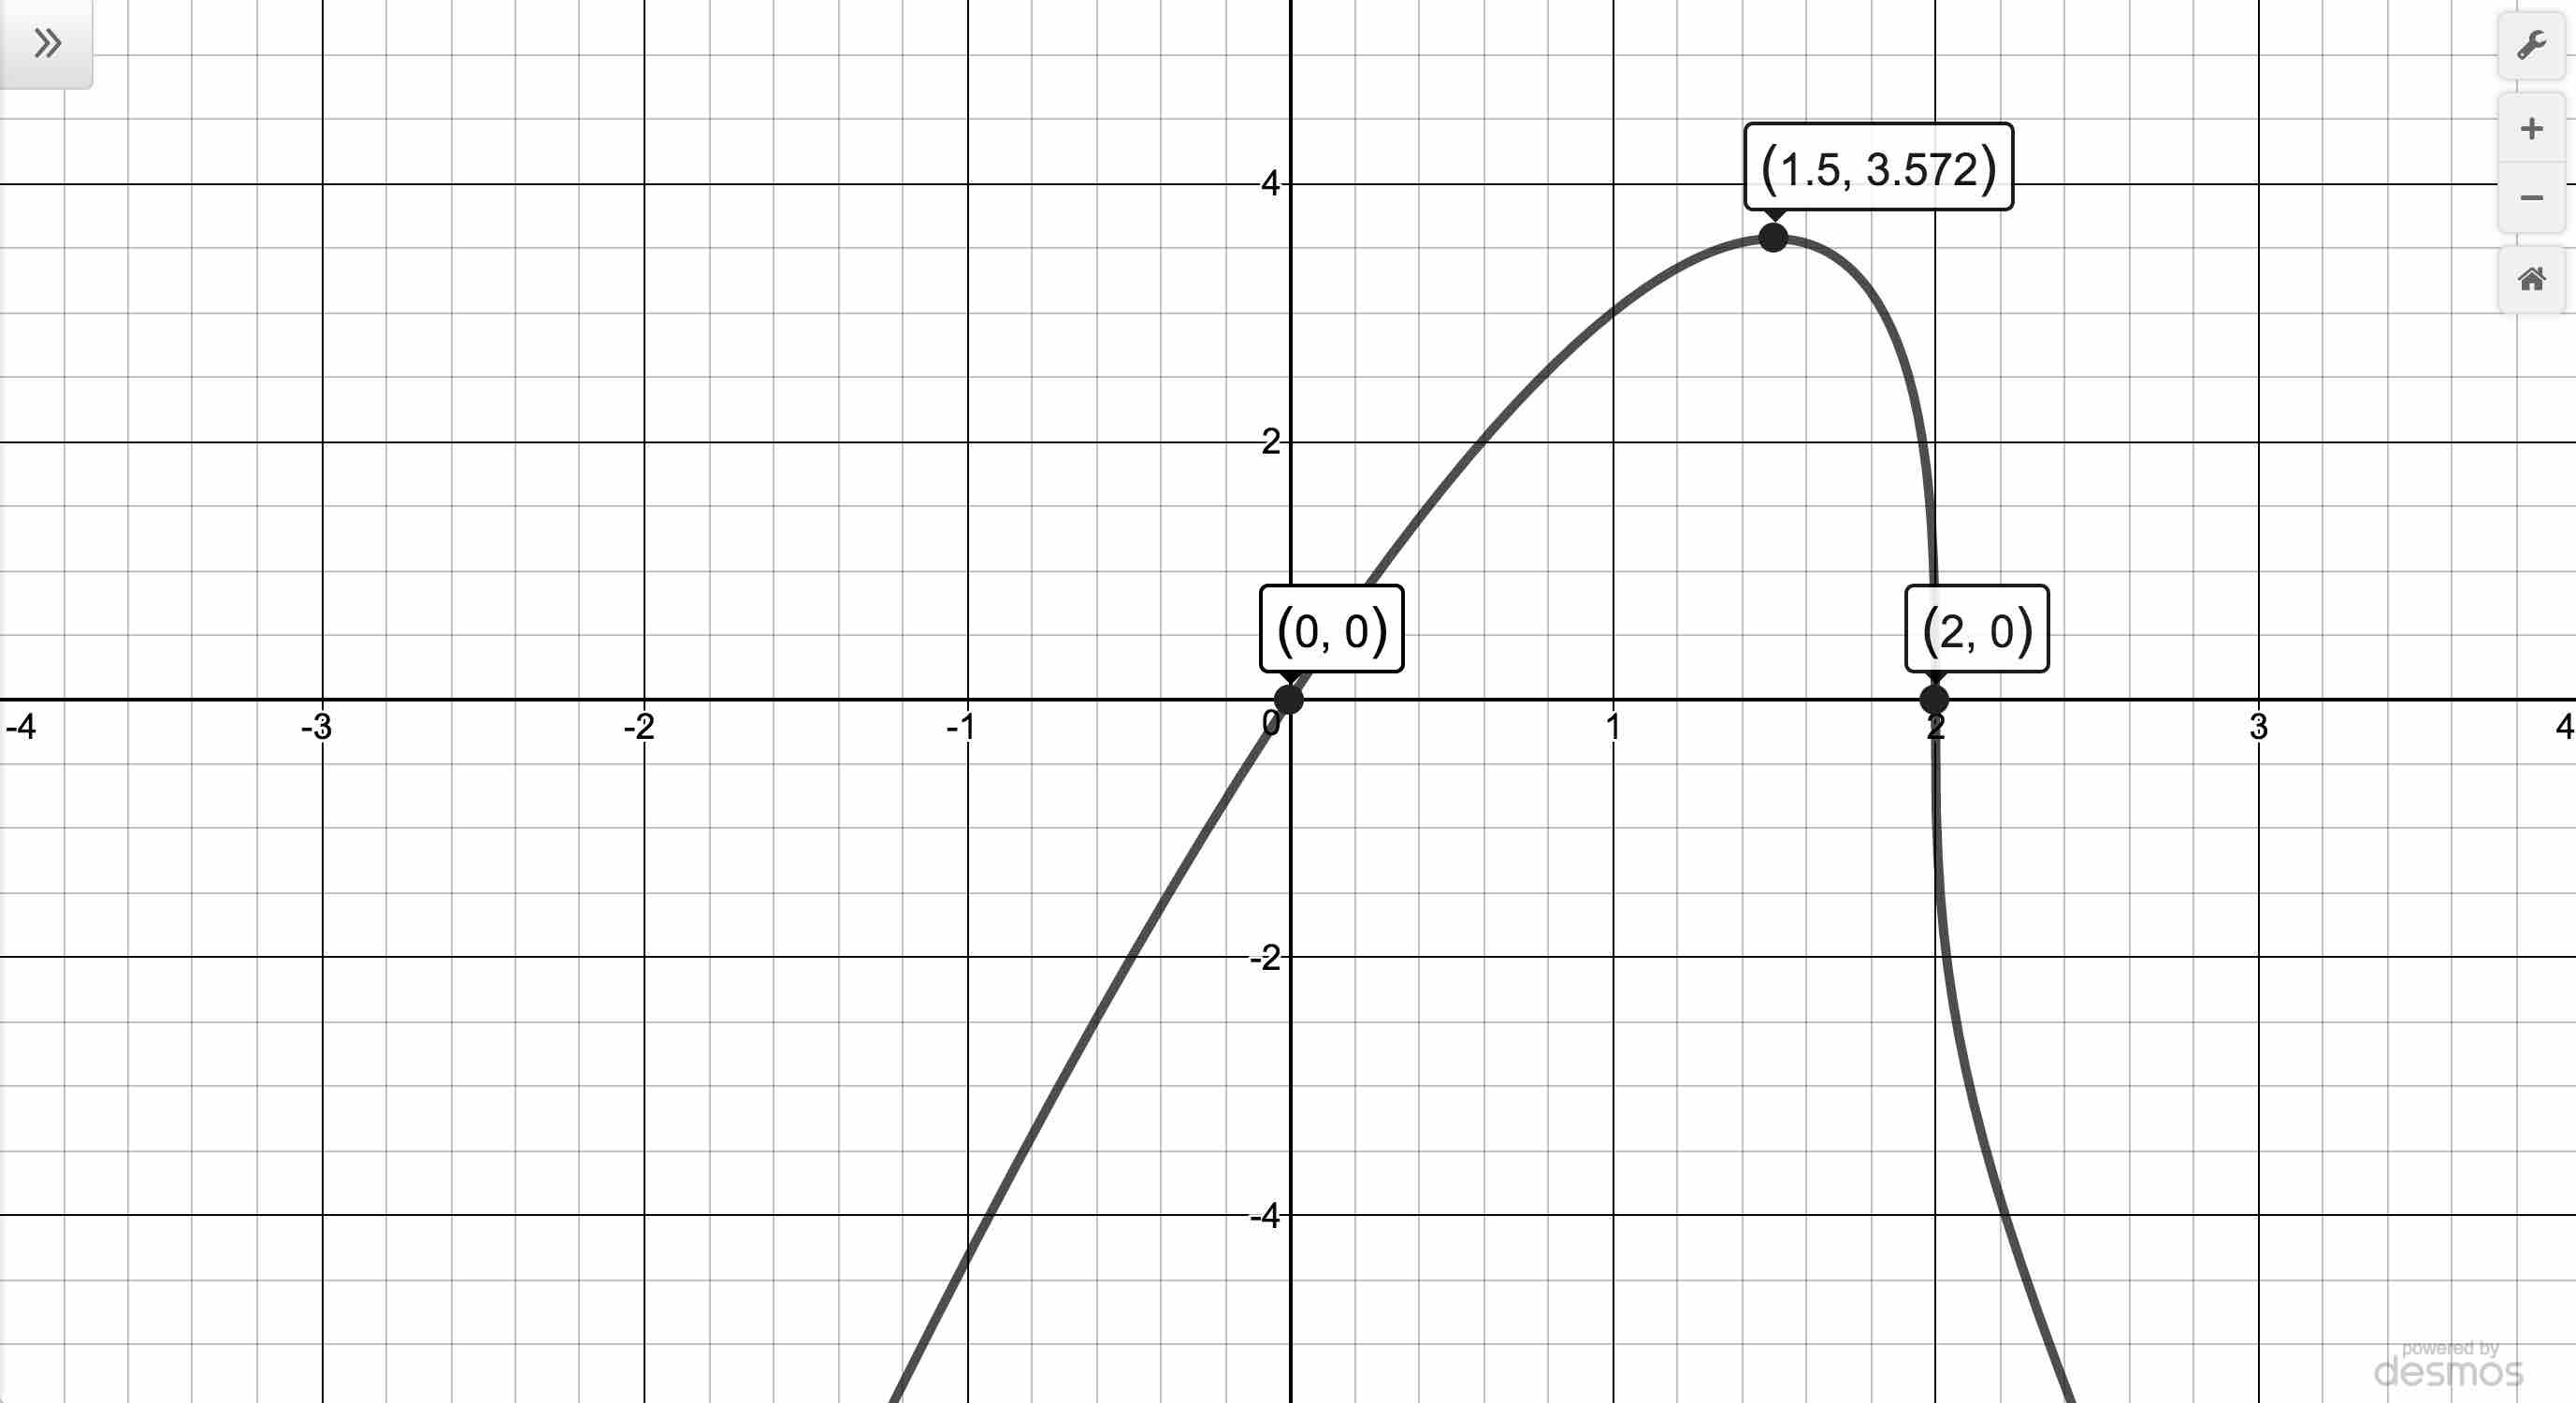
\includegraphics[width=3in]{./RootRadicalFunctionsGraphics/RadicalGraphEx01.jpg} &

\begin{mfpic}[20]{-4}{2}{-1}{1}
\arrow \reverse \arrow \polyline{(-4,0),(2,0)}
\xmarks{-2,0}
\tlabel[cc](-3, 0.5){$(-)$}
\tlabel[cc](-2,-0.5){$0$}
\tlabel[cc](-2,0.5){$0$}
\tlabel[cc](-1,0.5){$(+)$}
\tlabel[cc](0,-0.5){$2$}
\tlabel[cc](0,0.5){$0$}
\tlabel[cc](1,0.5){$(-)$}
\end{mfpic} \\

The graph of $y=f(x)$  \hspace{0.75in} & Sign Diagram for $f(x)$ \\


\end{tabular}
\end{center} 


\item  The index of the radical  in the expression for $g(t)$ is odd, so our only concern is the denominator.  Setting $t+1=0$ gives $t=-1$, which we exclude, so our domain is $\{ t \in \mathbb{R} \, | \, t \neq -1\}$ or using interval notation, $(-\infty, -1) \cup (-1, \infty)$.    If we take the time to analyze the behavior of $g$ near $t=-1$, we find that as $t \rightarrow -1^{-}$, $g(t) = \sqrt[3]{\frac{8t}{t+1}}  \approx \sqrt[3]{\frac{-8}{\text{small $(-)$}}}  \approx \sqrt[3]{\text{ big$(+)$}} = \text{big $(+)$}$.  That is, as $t \rightarrow -1^{-}$, $g(t) \rightarrow \infty$.  Likewise, as $t \rightarrow -1^{+}$, $g(t)  \approx \sqrt[3]{\frac{-8}{\text{small $(+)$}}}  \approx \sqrt[3]{\text{ big $(-)$}} = \text{big $(-)$}$.  This suggests as $t \rightarrow -1^{+}$, $g(t) \rightarrow -\infty$.  This behavior points to a vertical asymptote, $t=-1$.

To find the $t$-intercepts of the graph of $g$, we find the zeros of $g$ by setting $g(t) = \sqrt[3]{\frac{8t}{t+1}} = 0$.  Cubing both sides and clearing denominators  gives $8t = 0$ or $t = 0$.  Hence our  $t$-, and in this case,  $y$- intercept is $(0,0)$.

To determine the end behavior, we note that as $t \rightarrow \pm \infty$, $\frac{8t}{t+1} \rightarrow \frac{8}{1} = 8$.  Hence, it stands to reason that as $t\rightarrow \pm \infty$, $g(t) =  \sqrt[3]{\frac{8t}{t+1}} \rightarrow \sqrt[3]{8} = 2$.  This suggests the graph of $y = g(t)$ has a horizontal asymptote at $y = 2$.

We graph $y = g(t)$ below on the left. The graph confirms our suspicions about the asymptotes $t = -1$ and $y = 2$.  Moreover, the range appears to be $(-\infty, 2) \cup (2, \infty)$.  We could check if the graph ever crosses its horizontal asymptote by attempting to solve $g(t) =  \sqrt[3]{\frac{8t}{t+1}} = 2$.  Cubing both sides and clearing denominators gives $8t = 8(t+1)$ which gives $0 = 8$, a contradiction.  This proves $2$ is not in the range, as we had suspected. 

Scanning the graph,  there  appears to be no local extrema, and, moreover,  the graph suggests $g$  is increasing on $(-\infty, -1)$ and again on $(-1, \infty)$.  As with the previous example, the graph appears locally vertical near its intercept $(0,0)$.

\smallskip

To create a sign diagram for $g(t)$, we note that the function is undefined when $t = -1$ (so we place a `\textinterrobang' above it) and has a zero $t=0$.  When  $t<-1$, $g(t) > 0$ or $(+)$, for $-1<t<0$, $g(t)<0$ or $(-)$, and for $t>0$, $g(t) > 0$ or $(+)$.  Below on the right is a sign diagram for $g(t)$.

\begin{center}

\begin{tabular}{cc}

 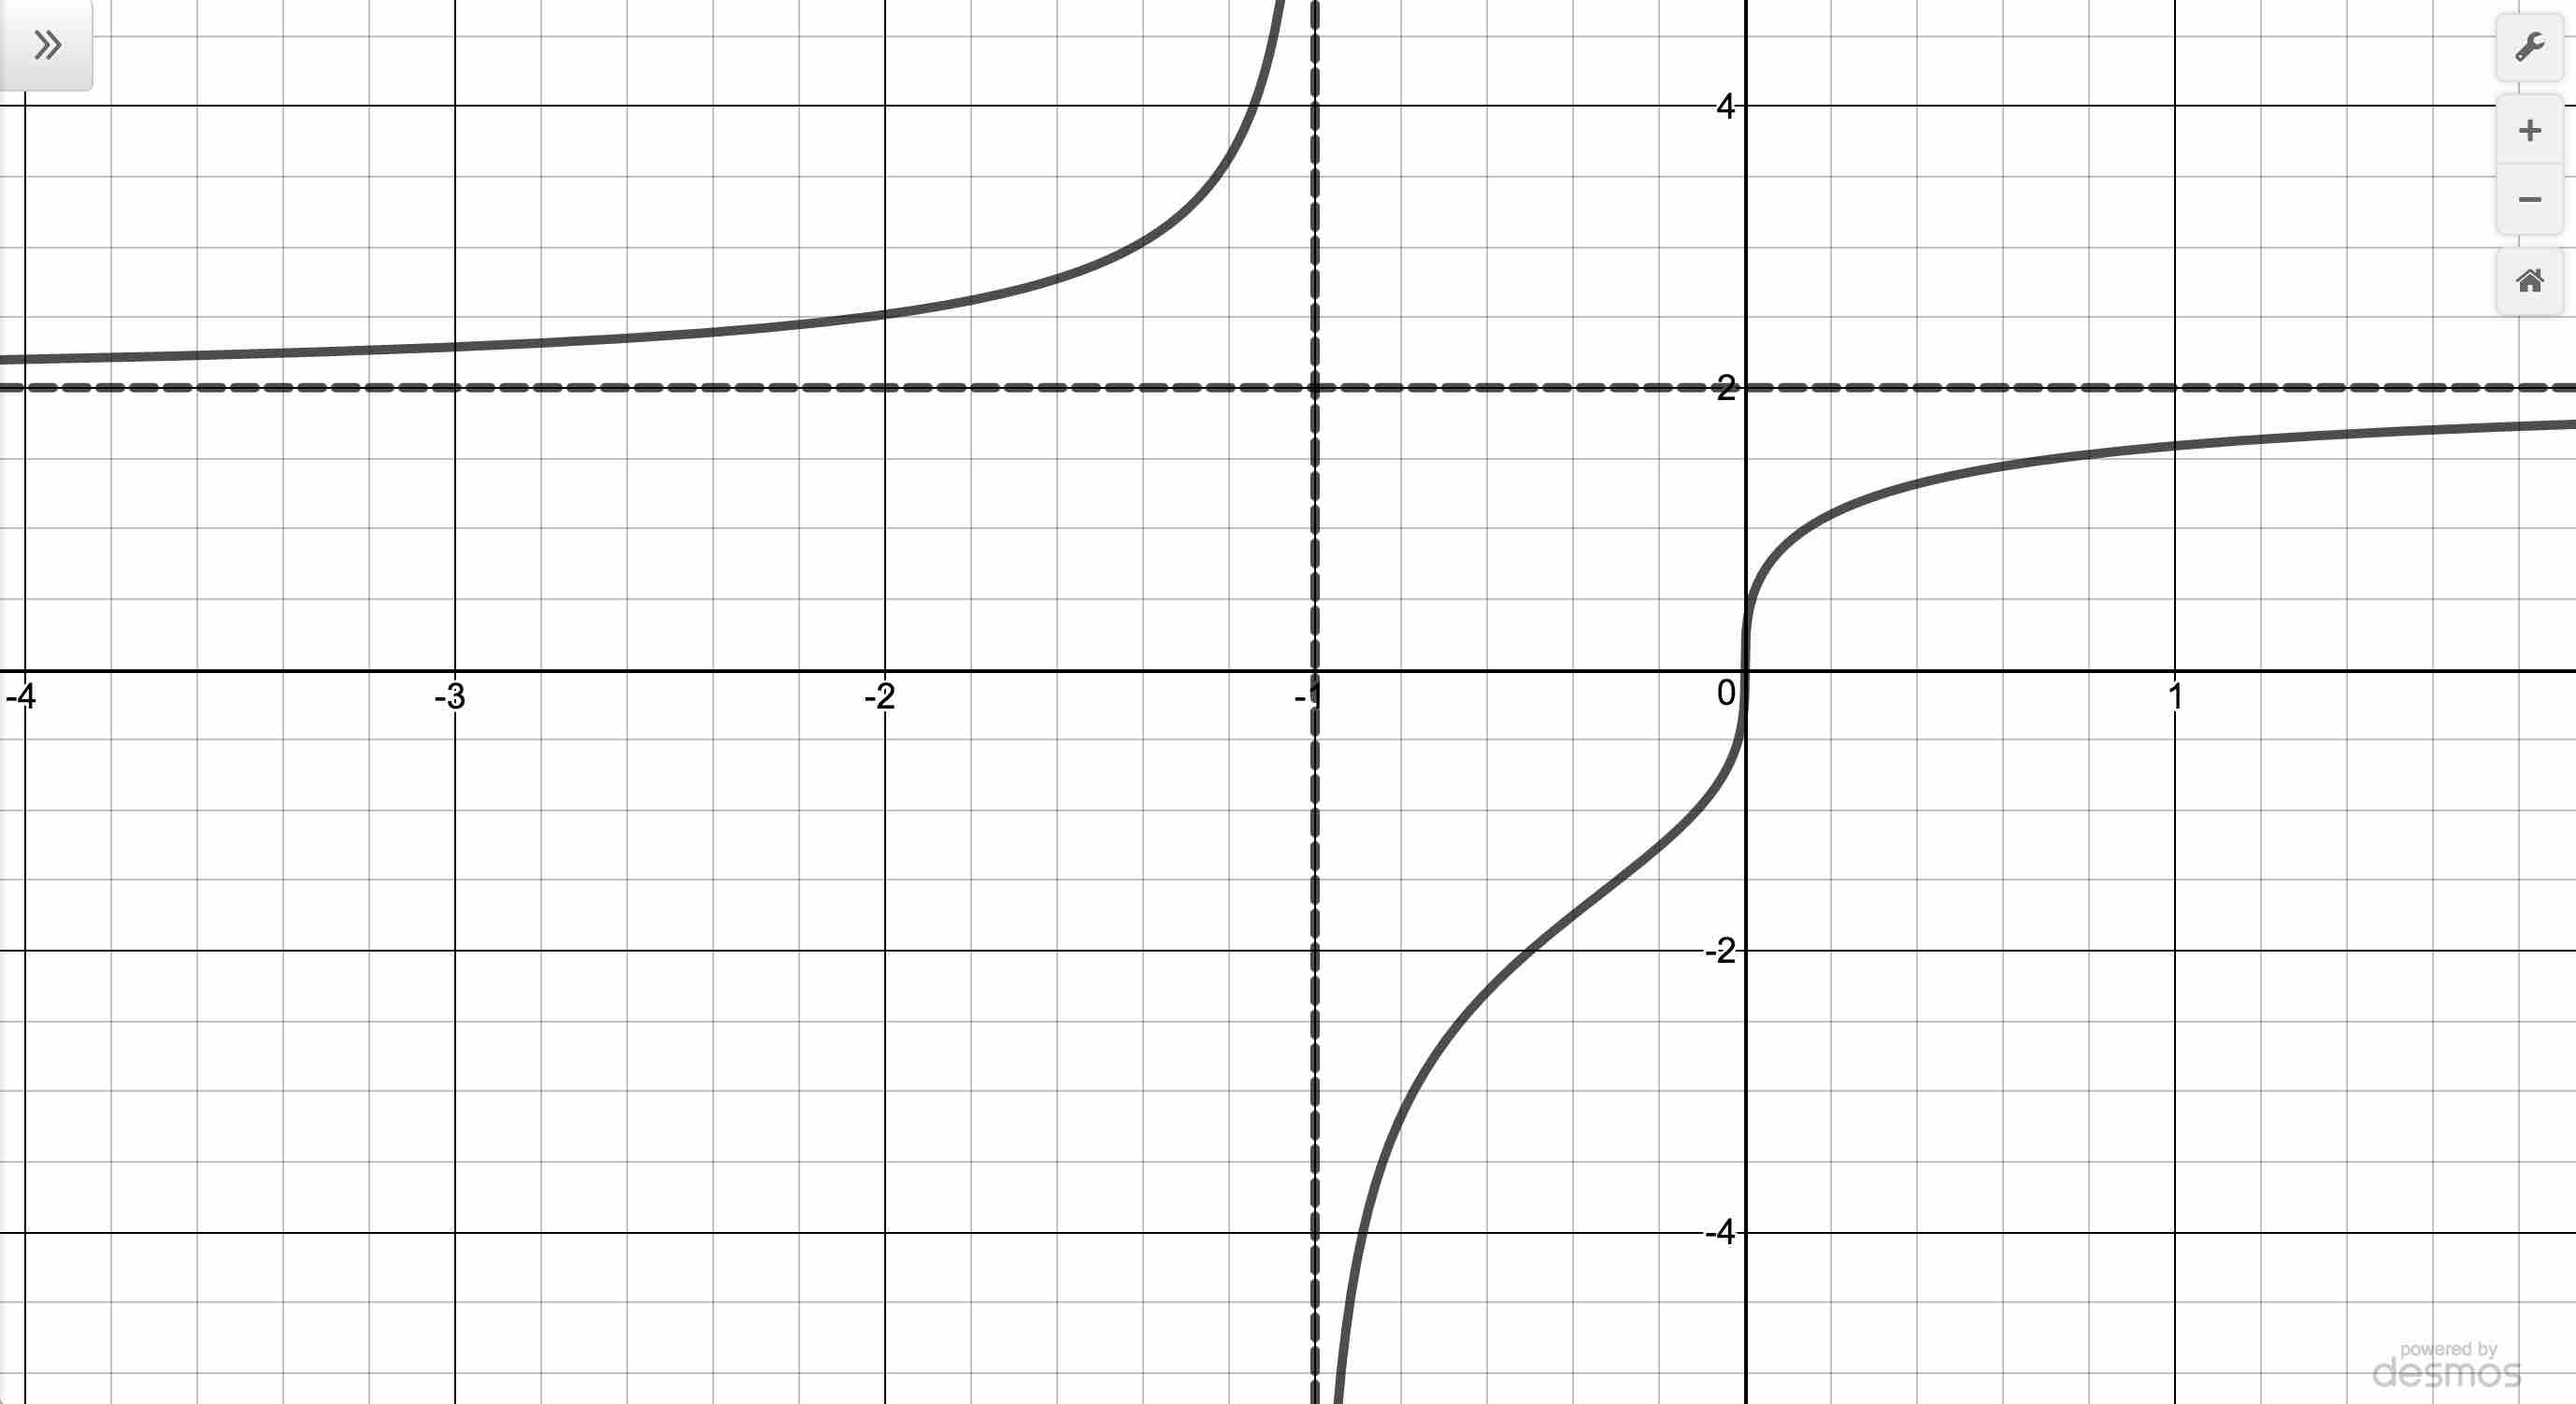
\includegraphics[width=3in]{./RootRadicalFunctionsGraphics/RadicalGraphEx02.jpg}  &
 
\begin{mfpic}[20]{-4}{2}{-1}{1}
\arrow \reverse \arrow \polyline{(-4,0),(2,0)}
\xmarks{-2,0}
\tlabel[cc](-3, 0.5){$(+)$}
\tlabel[cc](-2,-0.5){$-1 \hspace{7pt}$}
\tlabel[cc](-2,0.5){\textinterrobang}
\tlabel[cc](-1,0.5){$(-)$}
\tlabel[cc](0,-0.5){$0$}
\tlabel[cc](0,0.5){$0$}
\tlabel[cc](1,0.5){$(+)$}
\end{mfpic} \\

The graph of $y=g(t)$  \hspace{0.75in} & Sign Diagram for $g(t)$  \\


\end{tabular}
\end{center} 

 \item  The expression for $h(x) = \frac{3x}{\sqrt{x^2 + 1}}$ has both a denominator and an even-indexed radical, so we have to be extra cautious here.  Fortunately for us, the quantity $x^2+1 >0$ for al real numbers $x$. Not only does this mean $\sqrt{x^2+1}$ is always defined, it also tells us $\sqrt{x^2+1}>0$ for all $x$, too.  This means the domain of $h$ is all real numbers, $(-\infty, \infty)$.
 
Solving for the zeros of $h$ gives only $x = 0$, and we find, once again, $(0,0)$ is both our lone $x$- and $y$-intercept.  Moving on to end behavior, as $x \rightarrow \pm \infty$, the term $x^2$ is the dominant term in the radicand in the denominator. As such, $h(x) = \frac{3x}{\sqrt{x^2 + 1}} \approx \frac{3x}{\sqrt{x^2}} = \frac{3x}{|x|}$.  As $x \rightarrow \infty$, $|x| = x$ (since $x>0$), so $h(x) \approx \frac{3x}{x} = 3$, so $h(x) \rightarrow 3$.  Likewise, as $x \rightarrow -\infty$, $|x| = -x$ (since $x<0$) and hence, $h(x)\approx  \frac{3x}{-x} = -3$, so $h(x) \rightarrow -3$.  This analysis suggests the graph of $y=h(x)$ has not one, but \textit{two} horizontal asymptotes.\co{\footnote{We warned you this was coming \ldots see the discussion following Theorem \ref{hathm} in Section \ref{IntroRational}.}} The graph of $h$ below on the left bears this out.

From the graph, we see the range of $h$ appears to be $(-3,3)$.  Attempting to solve $h(x) = \frac{3x}{\sqrt{x^2 + 1}} = \pm 3$ gives, in either case, $9x^2 = 9(x^2+1)$ which reduces to $0 = 9$, a contradiction.  Hence, the graph of $y = h(x)$ never reaches its horizontal asymptotes. Moreover, $h$ appears to be always increasing, with no local extrema or `unusual' steepness.  One last remark:  it appears as if the graph of $h$ is symmetric about the origin.  We check $h(-x) = \frac{3(-x)}{\sqrt{(-x)^2+1}} = - \frac{3x}{\sqrt{x^2 + 1}} = -h(x)$ which verifies $h$ is odd.

\smallskip

Since the domain of $h$ is all real number and the only zero of $h$ is $x=0$, the sign diagram for $h(x)$ is fairly straight forward.  For $x<0$, $h(x)<0$ or $(-)$ and for $x>0$, $h(x) >0$ or $(+)$.  The sign diagram for $h(x)$ is below on the right.

\begin{center}

\begin{tabular}{cc}

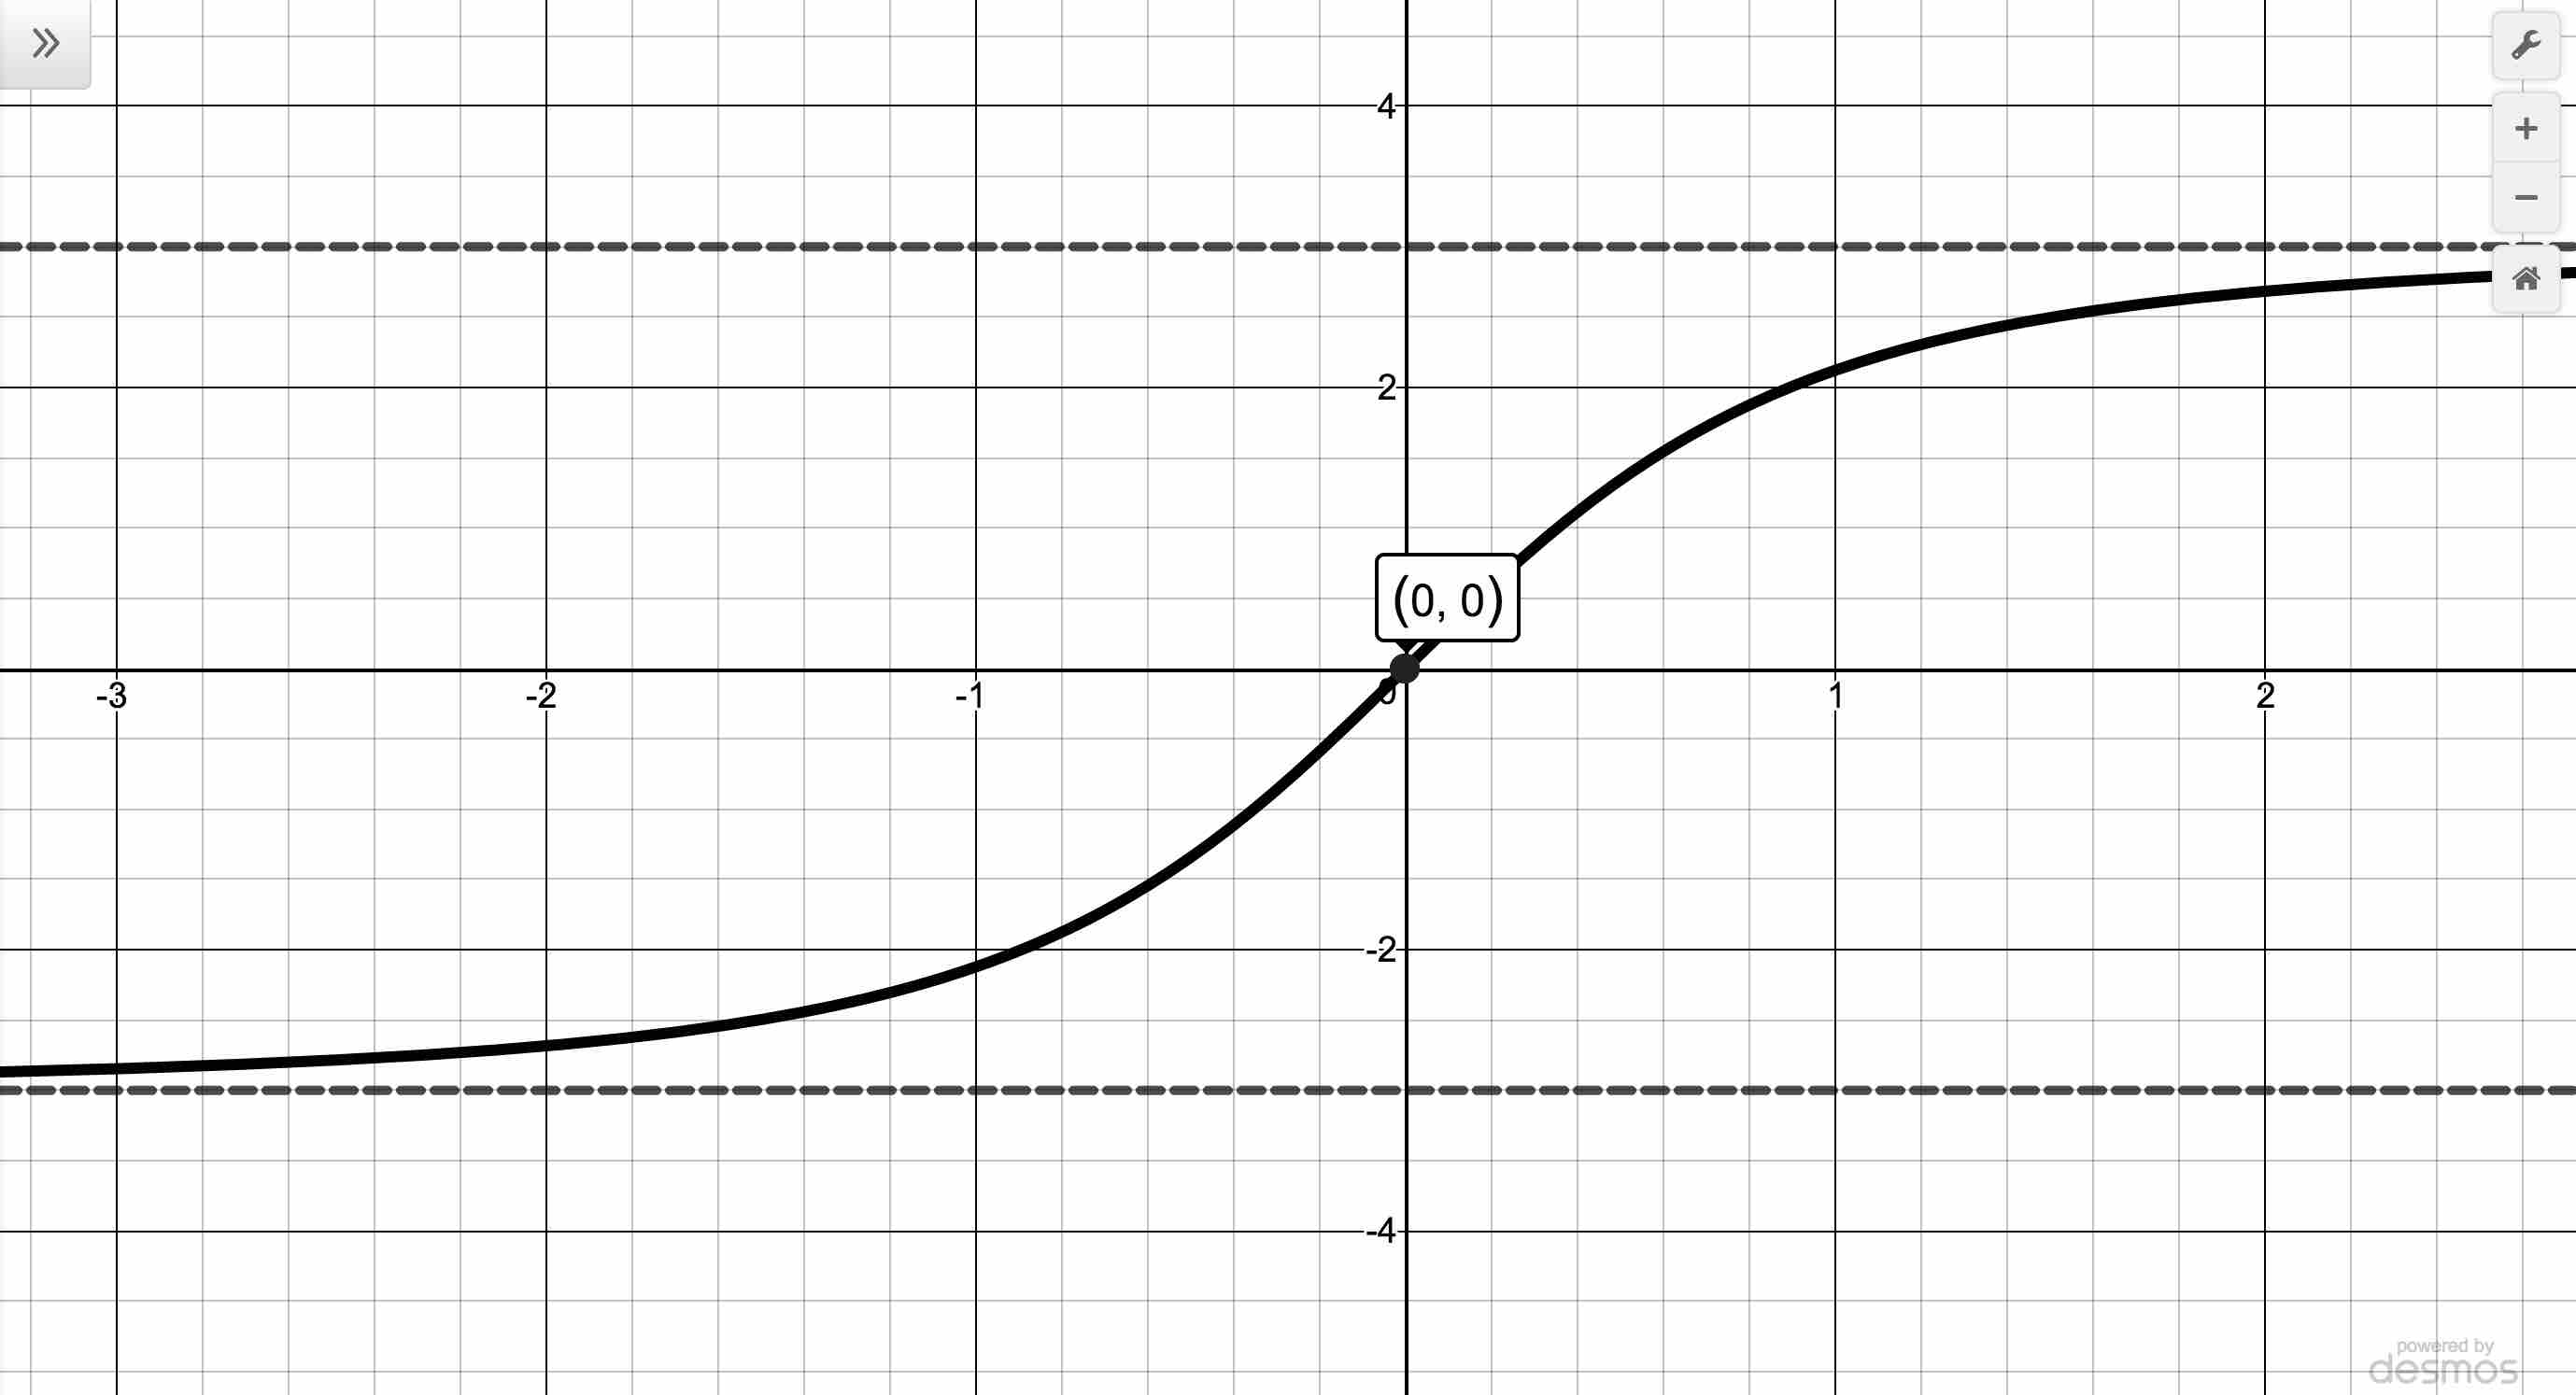
\includegraphics[width=3in]{./RootRadicalFunctionsGraphics/RadicalGraphEx03.jpg} &

\begin{mfpic}[20]{-4}{2}{-1}{1}
\arrow \reverse \arrow \polyline{(-2,0),(2,0)}
\xmarks{0}
\tlabel[cc](-1,0.5){$(-)$}
\tlabel[cc](0,-0.5){$0$}
\tlabel[cc](0,0.5){$0$}
\tlabel[cc](1,0.5){$(+)$}
\end{mfpic} \\

The graph of $y=h(x)$  \hspace{0.75in} & Sign Diagram for $h(x)$ \\


\end{tabular}
\end{center} 



\item  The first thing to note about the expression  $r(t) = t^{-1} \sqrt{16t^4-1}$ is that $t^{-1} = \frac{1}{t}$.  Hence, we must exclude $t=0$ from the domain straight away. Next, we have an even-indexed radical expression: $\sqrt{16t^4-1}$.  In order for this to return a real number, we require  $16t^4-1 \geq 0$.  Instead of using a sign diagram to solve this,\co{\footnote{See Section \ref{RealZeros}}} we opt instead to  \textit{carefully} use properties of radicals.  Isolating $t^4$, we have $t^4 \geq \frac{1}{16}$.  Since the root functions are increasing, we can apply the fourth root to both sides and preserve the inequality:  $\sqrt[4]{t^4} \geq \sqrt[4]{\frac{1}{16}}$ which gives\footnote{Recall: $\sqrt[n]{x^n} = |x|$, not $x$,  if $n$ is even.} $|t| \geq \frac{1}{2}$. Note that since $t =0$ does \textit{not} satisfy this inequality, restricting $t$ in this manner takes care of  \textit{both} domain issues, so the domain is  $\left(-\infty, -\frac{1}{2} \right] \cup \left[\frac{1}{2}, \infty \right)$. 

Next, we look for zeros.  Setting $r(t) = t^{-1} \sqrt{16t^4-1} = \frac{\sqrt{16t^4-1}}{t}=0$ gives $\sqrt{16t^4-1} = 0$.  After squaring both sides, we get $16t^4-1 = 0$ or $t^4 = \frac{1}{16}$.  Extracting fourth roots, we get $t = \pm \frac{1}{2}$. Both of these are (barely!) in the domain of $r$, so our $t$ intercepts are $\left( -\frac{1}{2}, 0\right)$ and $\left( \frac{1}{2}, 0\right)$.  Note, the graph of $r$ has no $y$-intercept, since $r(0)$ is undefined ($t=0$ is not in the domain of $r$).  

Concerning end behavior, we note the term $16t^4$ dominates the radicand $\sqrt{16t^4-1}$ as $t \rightarrow \pm \infty$,  hence, $r(t) = \frac{\sqrt{16t^4-1}}{t} \approx \frac{\sqrt{16t^4}}{t} = \frac{4t^2}{t} = 4t$.  This suggests the graph of $y = r(t)$ has a slant asymptote with slope $4$.\co{\footnote{Note: this analysis suggests the slant asymptote is $y = 4t+b$, but from this analysis, we cannot determine the value of $b$.  As with slant asymptotes in Section \ref{IntroRational}, we'd need to perform a more detailed analysis which we omit in this case owing to the complexity of the function.}}  

We graph $y=r(t)$ below on the left.  We see the range appears to be all real numbers, $(-\infty, \infty)$.  It appears as if $r$ is increasing on $\left(-\infty, -\frac{1}{2} \right]$ and again on $\left[\frac{1}{2}, \infty \right)$.  The graph does appear to be asymptotic to $y = 4t$, and it also appears to be symmetric about the origin.  Sure enough, we find  $r(-t) = \frac{\sqrt{16(-t)^4-1}}{-t}  = - \frac{\sqrt{16t^4-1}}{t} = -r(t)$, proving $r$ is an odd function.

\smallskip

To construct the sign diagram for $r(t)$ we note $r$ has two zeros, $t = \pm \frac{1}{2}$.  For $t < \frac{1}{2}$, $r(t) < 0$ or $(-)$ and when $t > \frac{1}{2}$, $r(t) > 0$ or $(+)$.  When $-\frac{1}{2} < t < \frac{1}{2}$, $r$ is undefined so we have removed that segment from the diagram, as seen below on the right.

\begin{center}

\begin{tabular}{cc}

 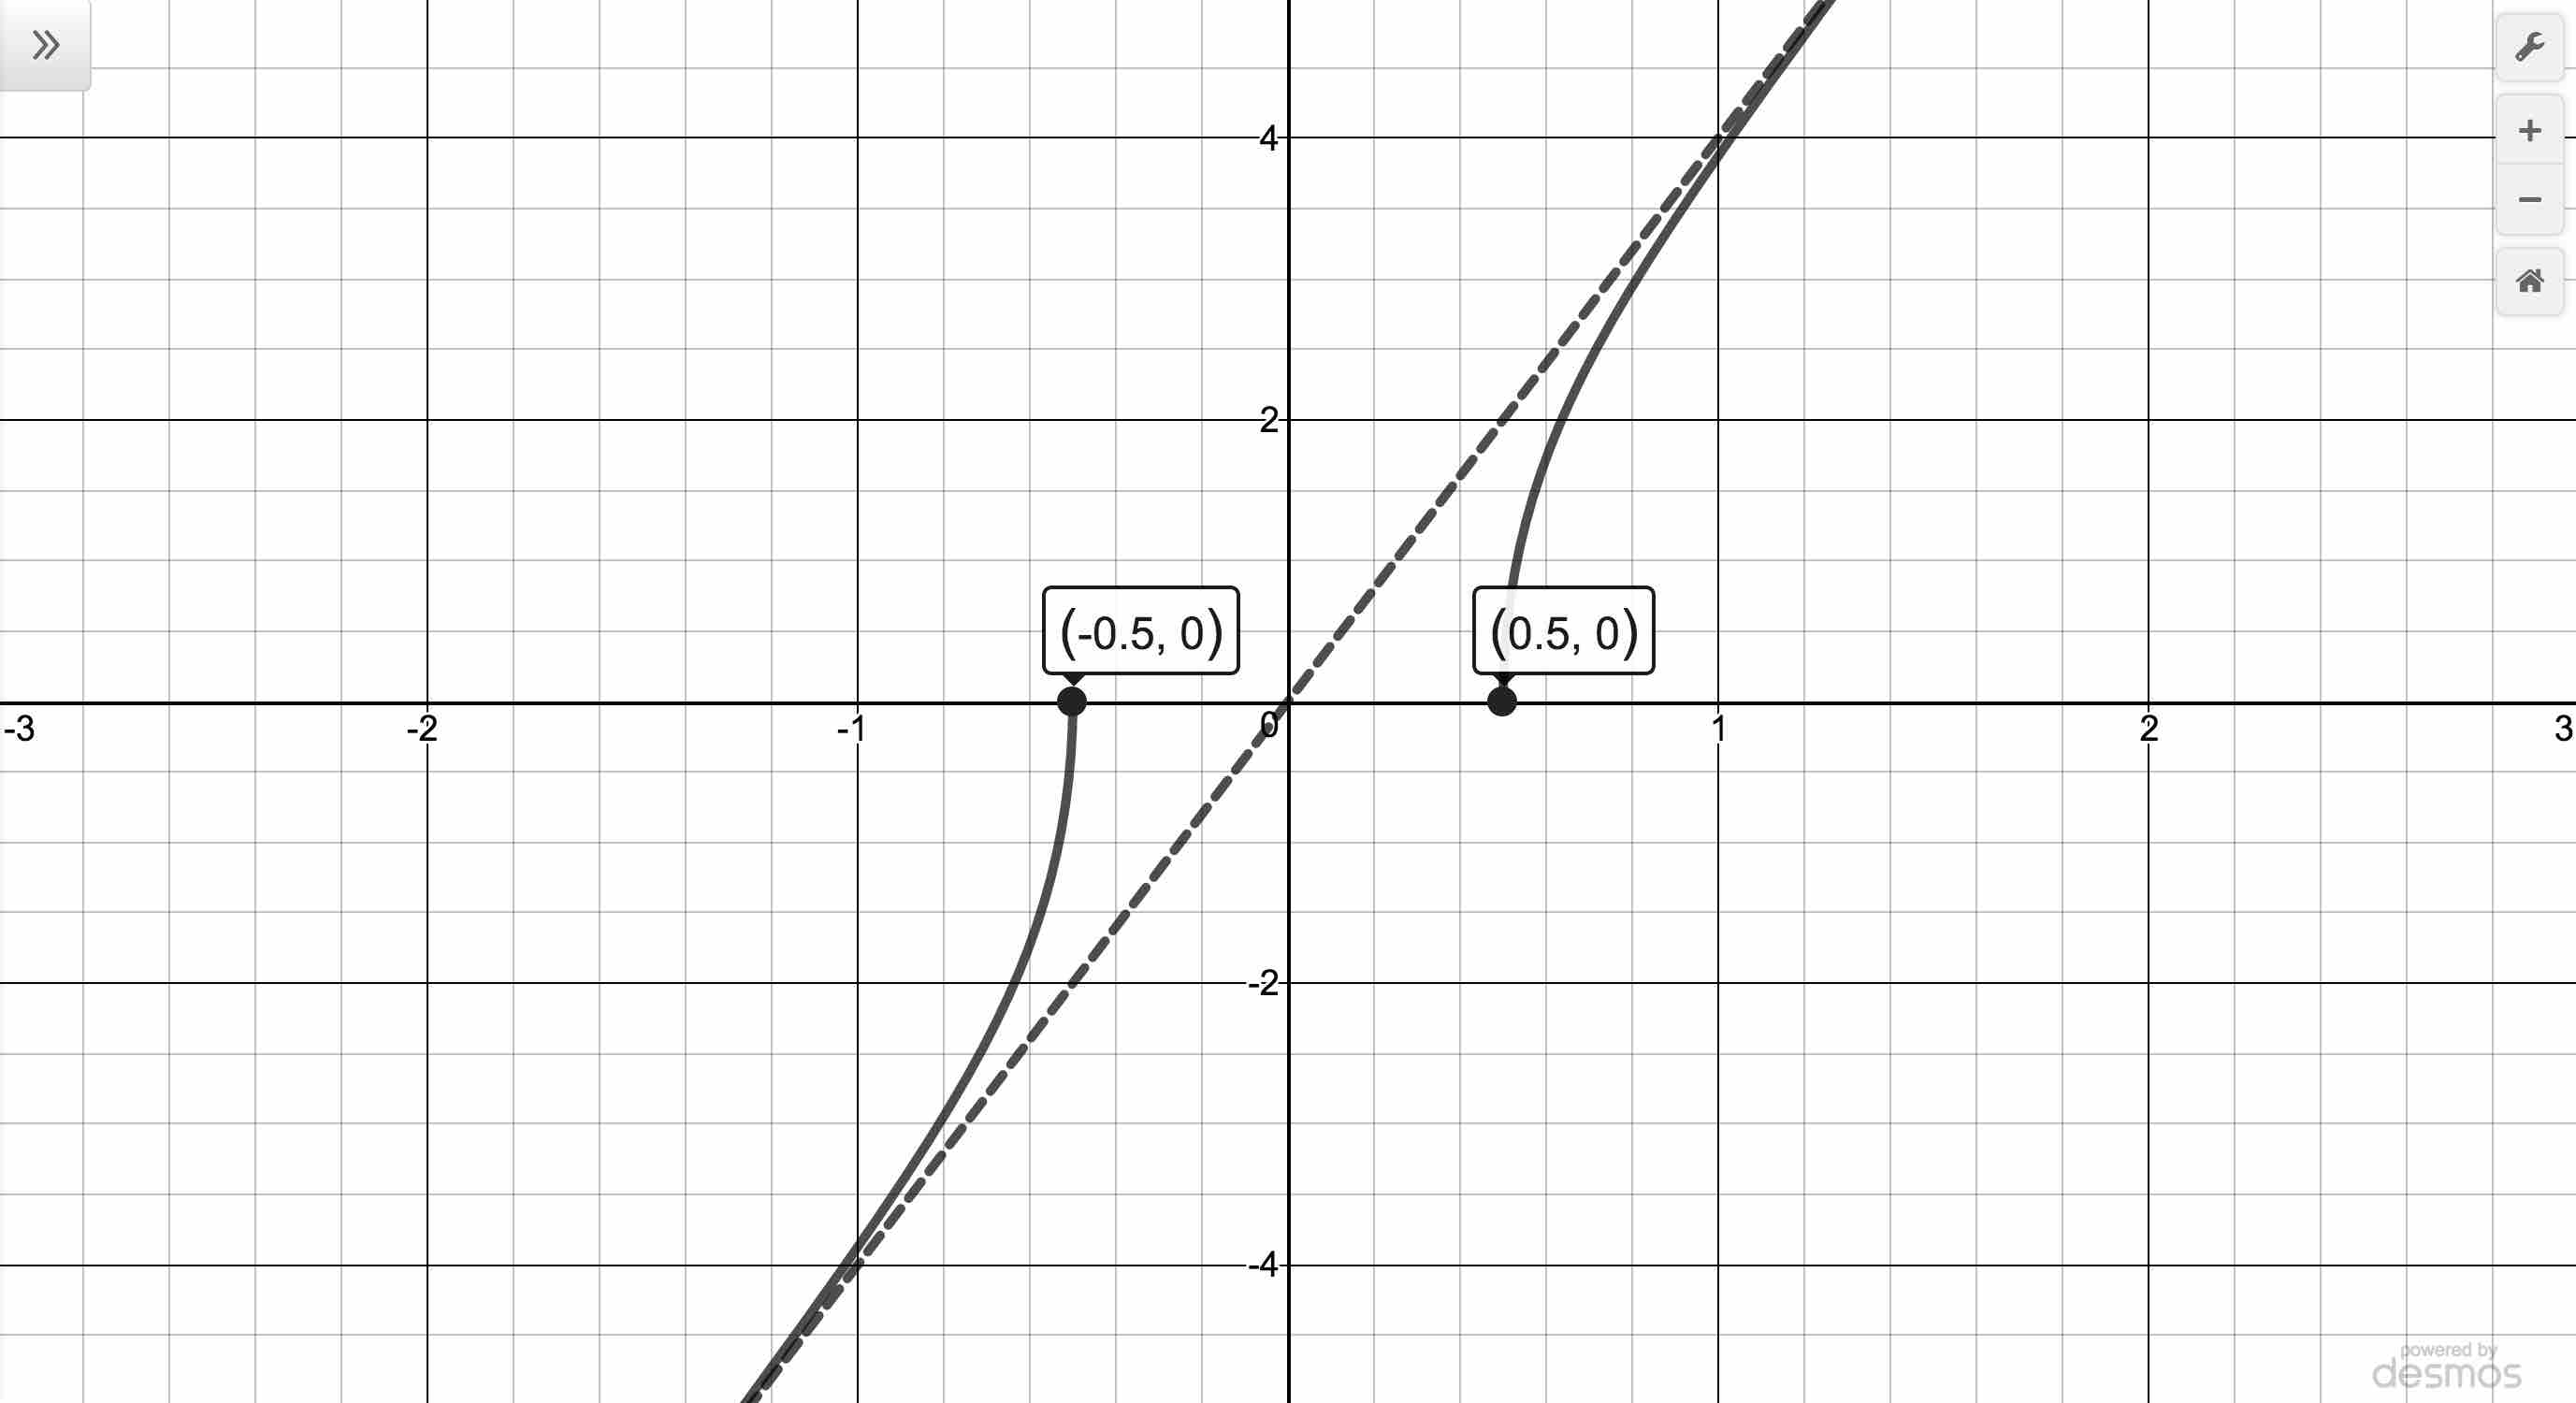
\includegraphics[width=3in]{./RootRadicalFunctionsGraphics/RadicalGraphEx04.jpg} &
  
 \begin{mfpic}[20][10]{0}{4}{-1.5}{1.5}
\arrow \polyline{(2,0), (0,0)}
\arrow \polyline{(3,0), (5,0)}
\xmarks{2,3}
\tlabel[cc](2,-1){$-\frac{1}{2} \hspace{7pt}$}
\tlabel[cc](1,1){$(-)$}
\tlabel[cc](4,1){$(+)$}
\tlabel[cc](2,1){$0$}
\tlabel[cc](3,1){$0$}
\tlabel[cc](3,-1){$\frac{1}{2}$}
\end{mfpic}
\\

The graph of $y=r(t)$  \hspace{0.75in} & Sign Diagram for $r(t)$. \\


\end{tabular}
\end{center} 



\qed
\end{enumerate}

\end{ex}

We end this section with a classic application of root functions.


\begin{ex} \label{SasquatchCable} Carl wishes to get high speed internet service installed in his remote Sasquatch observation post located $30$ miles from Route $117$. The nearest junction box is located $50$ miles down the road from the post, as indicated in the diagram below.  Suppose it costs $\$ 15$ per mile to run cable along the road and $\$ 20$ per mile to run cable off of the road.

\begin{enumerate}

\item   Find an expression $C(x)$ which computes the cost of connecting the Junction Box to the Outpost as a function of $x$, the number of miles the cable is run along Route $117$ before heading off road directly towards the Outpost.  Determine a reasonable applied domain for the problem.

\item  Use your calculator to graph $y=C(x)$ on its domain.  What is the minimum cost?  How far along Route $117$ should the cable be run before turning off of the road?

\end{enumerate}

\begin{center}
\begin{mfpic}[12]{-1}{15}{-1}{9}

\xmarks{0, 4}

\arrow \reverse \arrow \polyline{(0,8.75),(0,0.25)}

\arrow \reverse \arrow \polyline{(0.25,0),(3.75,0)}

\arrow \reverse \arrow \polyline{(4.25,0),(9.75,0)}

\arrow \reverse \arrow \polyline{(0,-1),(10,-1)}

\dashed \polyline{(4,0),(0,9)}

\point[3pt]{(0,9), (10,0)}

\tlabel[cc](1.25,9){\scriptsize Outpost}

\tlabel[cc](12,0){\scriptsize Junction Box}

\tlabel[cc](7,0.5){$x$}

\tlabel[cc](2,0.5){$y$}

\tlabel[cc](3,4.5){$z$}

\tlabel[cc](5,-.5){\scriptsize Route $117$}

\tlabel[cc](5,-2){\scriptsize $50$ miles}

\tlabel[cc](-0.5,0){\rotatebox{90}{\hspace{1.5in} \scriptsize $30$ miles}}

\end{mfpic}
\end{center}



{\bf Solution.}

\begin{enumerate}

\item  The cost is broken into two parts:  the cost to run cable along Route $117$ at $\$15$ per mile, and the cost to run it off road at $\$20$ per mile.  Since $x$ represents the miles of cable run along Route $117$, the cost  for that portion is $15x$.  
From the diagram, we see that the number of miles the cable is run off road is $z$, so the cost of that portion is $20z$.  Hence, the total cost is $15x + 20z$.  

\smallskip

Our next goal is to determine $z$ in terms of $x$.  The diagram suggests we can use the Pythagorean Theorem to get $y^2+30^2 = z^2$.  But we also see $x+y = 50$ so that $y=50-x$.  Substituting $(50-x)$ in for $y$ we obtain $z^2 = (50-x)^2+900$.  Solving for $z$, we obtain $z = \pm \sqrt{(50-x)^2+900}$.  Since $z$ represents a distance, we choose $z = \sqrt{(50-x)^2+900}$.

Hence, the cost as a function of $x$  is given by $C(x) = 15x + 20\sqrt{(50-x)^2+900}$.  From the context of the problem, we have $0 \leq x \leq 50$.

\item  We graph $y=C(x)$ below and find our (local) minimum to be at the point $(15.98, 1146.86)$.  Here the $x$-coordinate tells us that in order to minimize cost, we should run $15.98$ miles of cable along Route 117 and then turn off of the road and head towards the outpost. The $y$-coordinate tells us that the minimum cost, in dollars, to do so is $\$1146.86$.  The ability to stream live SasquatchCasts?  Priceless.

\medskip

\centerline{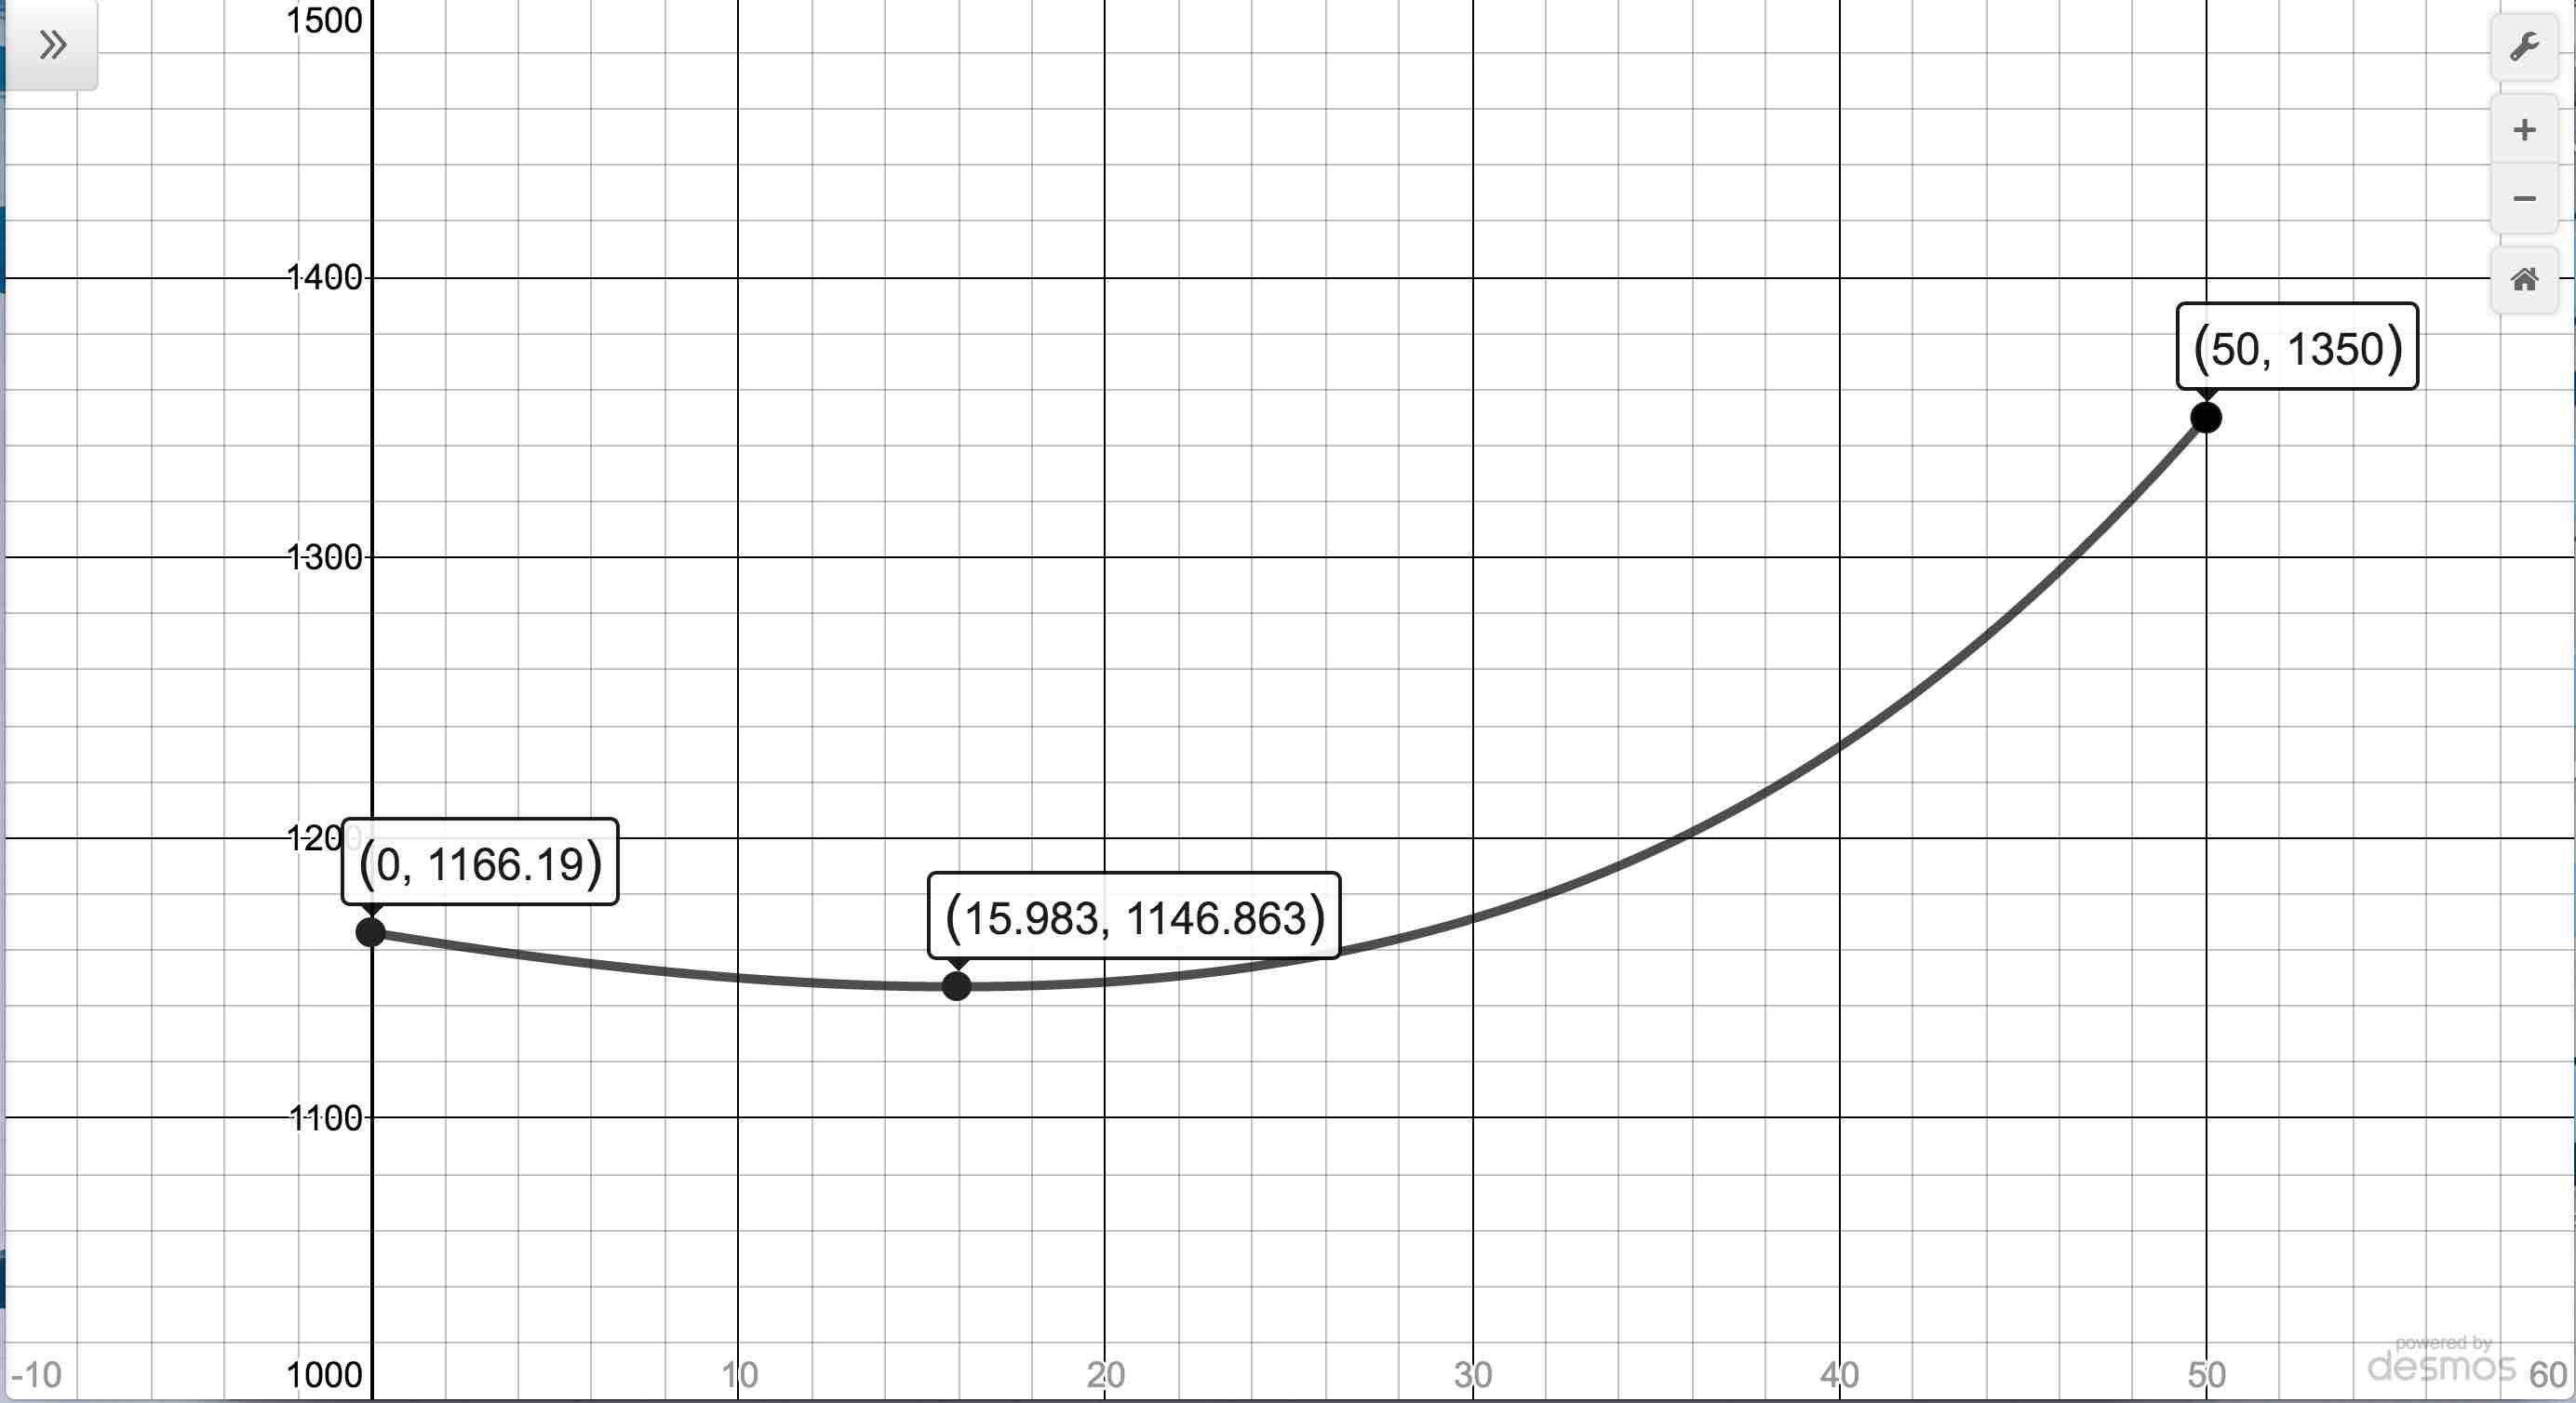
\includegraphics[width=4in]{./RootRadicalFunctionsGraphics/CostCableEx.jpg}}


 \qed

\end{enumerate}

\end{ex}

\newpage

\subsection{Exercises}

In Exercises \ref{radicalgraphexfirst} - \ref{radicalgraphexlast},  given the pair of functions $f$ and $F$, sketch the graph of $y=F(x)$ by starting with the graph of $y = f(x)$ and using Theorem \ref{linearrootgraphs}.   Track at least two points and state the domain and range using interval notation.

\begin{multicols}{2}
\begin{enumerate}

\item $f(x) = \sqrt{x}$, $F(x) = \sqrt{x+3}-2$ \label{radicalgraphexfirst}
\item $f(x) = \sqrt{x}$, $F(x) = \sqrt{4-x}-1$ 

\setcounter{HW}{\value{enumi}}
\end{enumerate}
\end{multicols}

\begin{multicols}{2}
\begin{enumerate}
\setcounter{enumi}{\value{HW}}
\item $f(x) = \sqrt[3]{x}$, $F(x) = \sqrt[3]{x-1}-2$ 
\item $f(x) = \sqrt[3]{x}$, $F(x) = -\sqrt[3]{8x + 8} + 4$ 

\setcounter{HW}{\value{enumi}}
\end{enumerate}
\end{multicols}

\begin{multicols}{2}
\begin{enumerate}
\setcounter{enumi}{\value{HW}}

\item $f(x) = \sqrt[4]{x}$, $F(x) = \sqrt[4]{x-1}-2$
\item $f(x) = \sqrt[4]{x}$, $F(x) = -3\sqrt[4]{x - 7} +1$

\setcounter{HW}{\value{enumi}}
\end{enumerate}
\end{multicols}

\begin{multicols}{2}
\begin{enumerate}
\setcounter{enumi}{\value{HW}}

\item $f(x) = \sqrt[5]{x}$, $F(x) = \sqrt[5]{x + 2} + 3$
\item $f(x) = \sqrt[8]{x}$, $F(x) = \sqrt[8]{-x} - 2$ \label{radicalgraphexlast}
\setcounter{HW}{\value{enumi}}
\end{enumerate}
\end{multicols}

In Exercises \ref{findformulaforsqrtgraphfirst} - \ref{findformulaforsqrtgraphlast}, find a formula for each function below in the form $F(x) = a\sqrt{bx-h}+k$.

\smallskip

\textbf{NOTE:}  There may be more than one solution!

\begin{multicols}{2}

\begin{enumerate}
\setcounter{enumi}{\value{HW}}

\item $~$ \label{findformulaforsqrtgraphfirst}  $y=F(x)$ %$F(x) = -\sqrt{x+4}+2$

\begin{mfpic}[15]{-5}{5}{-1}{5}
\axes
\tlabel[cc](5,-0.5){\scriptsize $x$}
\tlabel[cc](0.5,5){\scriptsize $y$}
\tlabel[cc](-4, 2.5){\scriptsize $(-4,2)$}
%\tlabel[cc](-0.5,-1){\scriptsize $\left(0, \frac{1}{2} \right)$}
\xmarks{-4,-3,-2,-1,1,2,3,4}
\ymarks{1,2,3,4}
\tlpointsep{4pt}
\scriptsize
\axislabels {x}{ {$-4 \hspace{7pt}$} -4, {$-3 \hspace{7pt}$} -3, {$-2 \hspace{7pt}$} -2, {$-1 \hspace{7pt}$} -1,  {$3$} 3, {$4$} 4}
\axislabels {y}{{$1$} 1, {$2$} 2, {$3$} 3, {$4$} 4}
\penwd{1.25pt}
\arrow  \function{-4,5,0.1}{2-sqrt(x+4)}
\point[4pt]{(-4,2), (0,0)}
\tcaption{ \scriptsize $x$,$y$-intercept $(0,0)$}
\normalsize
\end{mfpic} 



\item $~$ \label{findformulaforsqrtgraphlast} $y = F(x)$ %$F(x) =2\sqrt{-x+1}$

\begin{mfpic}[15]{-5}{5}{-1}{5}
\axes
\tlabel[cc](5,-0.5){\scriptsize $x$}
\tlabel[cc](0.5,5){\scriptsize $y$}
%\tlabel[cc](-1.5, 0.5){\scriptsize $(-1,0)$}
%\tlabel[cc](-0.5,-1){\scriptsize $\left(0, \frac{1}{2} \right)$}
\xmarks{-4,-3,-2,-1,1,2,3,4}
\ymarks{1,2,3,4}
\tlpointsep{4pt}
\scriptsize
\axislabels {x}{ {$-4 \hspace{7pt}$} -4, {$-3 \hspace{7pt}$} -3, {$-2 \hspace{7pt}$} -2, {$-1 \hspace{7pt}$} -1, {$1$} 1, {$2$} 2, {$3$} 3, {$4$} 4}
\axislabels {y}{{$1$} 1, {$2$} 2, {$3$} 3, {$4$} 4}
\penwd{1.25pt}
\arrow \reverse \function{-5,1,0.1}{2*sqrt(1-x)}
\point[4pt]{(1,0), (0,2)}
\tcaption{ \scriptsize $x$-intercept $(1,0)$, $y$-intercept $(0,2)$}
\normalsize
\end{mfpic} 


\setcounter{HW}{\value{enumi}}

\end{enumerate}

\end{multicols}

In Exercises \ref{findformulaforcubedrootgraphfirst} - \ref{findformulaforcubedrootgraphlast}, find a formula for each function below in the form $F(x) = a\sqrt[3]{bx-h}+k$.

\smallskip

\textbf{NOTE:}  There may be more than one solution!

\begin{multicols}{2}
\begin{enumerate}
\setcounter{enumi}{\value{HW}}

\item $~$ \label{findformulaforcubedrootgraphfirst}  $y=F(x)$ %$F(x) = -\sqrt[3]{2x+1}$

\begin{mfpic}[15]{-5}{5}{-5}{5}
\axes
\tlabel[cc](5,-0.5){\scriptsize $x$}
\tlabel[cc](0.5,5){\scriptsize $y$}
\tlabel[cc](-1, 1.75){\scriptsize $(-1,1)$}
%\tlabel[cc](-0.5,-1){\scriptsize $\left(0, \frac{1}{2} \right)$}
\xmarks{-4,-3,-2,-1,1,2,3,4}
\ymarks{-4,-3,-2, -1, 1,2,3,4}
\tlpointsep{4pt}
\scriptsize
\axislabels {x}{ {$-4 \hspace{7pt}$} -4, {$-3 \hspace{7pt}$} -3, {$-2 \hspace{7pt}$} -2, {$-1 \hspace{7pt}$} -1,  {$3$} 3, {$4$} 4}
\axislabels {y}{{$-1$} -1, {$3$} 3, {$4$} 4, {$-2$} -2, {$-3$} -3, {$-4$} -4}
\penwd{1.25pt}
 \arrow \reverse \arrow \parafcn{-2.25,2,0.1}{((0-0.5*(t**3))-0.5,t)}
\point[4pt]{(-0.5,0), (0,-1), (-1,1)}
\tcaption{ \scriptsize $x$-intercept $\left(-\frac{1}{2}, 0\right)$,$y$-intercept $(0,-1)$}
\normalsize
\end{mfpic} 



\item $~$ \label{findformulaforcubedrootgraphlast} $y = F(x)$ %$F(x) =2\sqrt[3]{x-1}-2$

\begin{mfpic}[15]{-5}{5}{-5}{5}
\axes
\tlabel[cc](5,-0.5){\scriptsize $x$}
\tlabel[cc](0.5,5){\scriptsize $y$}
\tlabel[cc](2, -2){\scriptsize $(1,-2)$}
\xmarks{-4,-3,-2,-1,1,2,3,4}
\ymarks{-4,-3,-2, -1, 1,2,3,4}
\tlpointsep{4pt}
\scriptsize
\axislabels {x}{ {$-4 \hspace{7pt}$} -4, {$-3 \hspace{7pt}$} -3, {$-2 \hspace{7pt}$} -2, {$-1 \hspace{7pt}$} -1, {$1$} 1, {$2$} 2, {$3$} 3, {$4$} 4}
\axislabels {y}{{$-1$} -1,{$1$} 1, {$2$} 2, {$3$} 3, {$4$} 4, {$-2$} -2, {$-3$} -3, {$-4$} -4}
\penwd{1.25pt}
 \arrow \reverse \arrow \parafcn{-5,1,0.1}{(  (0.125*((t+2)**3))+1 ,t)}
\point[4pt]{(2,0), (0,-4), (1,-2)}
\tcaption{ \scriptsize $x$-intercept $(2,0)$, $y$-intercept $(0,-4)$}
\normalsize
\end{mfpic} 


\setcounter{HW}{\value{enumi}}
\end{enumerate}
\end{multicols}

\begin{enumerate}
\setcounter{enumi}{\value{HW}}



\item  \label{rootstosolvepolyineq} Use the fact that the $n$th root functions are increasing to solve the following polynomial inequalities:

\begin{multicols}{3}

\begin{enumerate}

\item  $x^3 \leq 64$  \vphantom{$\dfrac{(2x+1)^3}{4} < 2$ }  % $(-\infty, 4]$

\item  $2 - t^5 <  34$  \vphantom{$\dfrac{(2x+1)^3}{4} < 2$ }  % $(-2, \infty)$

\item $\dfrac{(2z+1)^3}{4} \geq 2$ % $\left[ -\frac{1}{2}, \infty \right)$

\setcounter{HWindent}{\value{enumii}}

\end{enumerate}
\end{multicols}

For the following inequalities, remember $\sqrt[n]{x^{n}} = |x|$ if $n$ is even:

\begin{multicols}{3}

\begin{enumerate}
\setcounter{enumii}{\value{HWindent}}

\item  $x^4 \leq 16$  \vphantom{$\dfrac{(2x+1)^3}{4} < 2$ }  % $[-2,2]$

\item  $6-t^6 < -58$  \vphantom{$\dfrac{(2x+1)^3}{4} < 2$ }  % $(-\infty, -2) \cup (2, \infty)$

\item $\dfrac{(2z+1)^4}{3} \geq 27$ % $(-\infty, -2] \cup [1, \infty)$

\end{enumerate}

\end{multicols}

\setcounter{HW}{\value{enumi}}
\end{enumerate}


For each function in Exercises \ref{algfcngraphexfirst} - \ref{algfcngraphexlast} below 

\begin{itemize}

\item Analytically:

\begin{multicols}{3}

\begin{itemize}

\item find the domain.

\item find the axis intercepts.

\item analyze the end behavior.

\end{itemize}

\end{multicols}

\item Graph the function with help from a graphing utility and determine:

\begin{multicols}{2}

\begin{itemize}

\item  the range.

\item the local extrema, if they exist.

\end{itemize}

\end{multicols}

\begin{multicols}{2}

\begin{itemize}

\item intervals of increase/decrease.

\item any `unusual steepness' or `local' verticality.

\end{itemize}

\end{multicols}

\begin{multicols}{2}

\begin{itemize}

\item  vertical asymptotes.

\item  horizontal / slant asymptotes.

\end{itemize}

\end{multicols}

\item Construct a sign diagram for each function using the intercepts and graph.

\item  Comment on any observed symmetry.


\end{itemize}

\begin{multicols}{2}
\begin{enumerate}
\setcounter{enumi}{\value{HW}}
\item $f(x) = \sqrt{1 - x^{2}}$ \label{algfcngraphexfirst}
\item $f(x) = \sqrt{x^2-1}$

\setcounter{HW}{\value{enumi}}
\end{enumerate}
\end{multicols}

\begin{multicols}{2}
\begin{enumerate}
\setcounter{enumi}{\value{HW}}

\item $g(t) = t \sqrt{1-t^2}$
\item $g(t) = t \sqrt{t^2-1}$

\setcounter{HW}{\value{enumi}}
\end{enumerate}
\end{multicols}

\begin{multicols}{2}
\begin{enumerate}
\setcounter{enumi}{\value{HW}}

\item $f(x) = \sqrt[4]{\dfrac{16x}{x^{2} - 9}}$
\item $f(x) = \dfrac{5x}{\sqrt[3]{x^{3} + 8}}$
\setcounter{HW}{\value{enumi}}
\end{enumerate}
\end{multicols}


\begin{multicols}{2}
\begin{enumerate}
\setcounter{enumi}{\value{HW}}

\item $g(t) = \sqrt{t(t + 5)(t - 4)}$
\item $g(t) = \sqrt[3]{t^{3} + 3t^{2} - 6t - 8}$ \label{algfcngraphexlast}

\setcounter{HW}{\value{enumi}}
\end{enumerate}
\end{multicols}



\begin{enumerate}
\setcounter{enumi}{\value{HW}}

\item  Rework Example \ref{SasquatchCable} so that the outpost is 10 miles from Route 117 and the nearest junction box is 30 miles down the road for the post.


\item  The volume $V$ of a right cylindrical cone depends on the radius of its base $r$ and its height $h$ and is given by the formula $V = \frac{1}{3} \pi r^2 h$.  The surface area $S$ of a right cylindrical cone also depends on $r$ and $h$ according to the formula $S = \pi r \sqrt{r^2+h^2}$.  In the following problems, suppose a cone is to have a volume of 100 cubic centimeters. 

\begin{enumerate}

\item  \label{heightintermsofr} Use the formula for volume to find the height as a function of $r$, $h(r)$.
\item  Use the formula for surface area along with  your answer to \ref{heightintermsofr} to find the surface area as a function of $r$, $S(r)$.
\item  Use your calculator to find the values of $r$ and $h$ which minimize the surface area.  What is the minimum surface area?  Round your answers to two decimal places.

\end{enumerate}


\item \label{pendulumproblem} The period of a pendulum in seconds is given by \[T = 2\pi \sqrt{\dfrac{L}{g}}\](for small displacements) where $L$ is the length of the pendulum in meters and $g = 9.8$ meters per second per second is the acceleration due to gravity.  My Seth-Thomas antique schoolhouse clock needs $T = \frac{1}{2}$ second and I can adjust the length of the pendulum via a small dial on the bottom of the bob.  At what length should I set the pendulum?


\item According to Einstein's Theory of Special Relativity, the observed mass  of an object is a function of how fast the object is traveling.  Specifically, if  $m_{r}$ is the mass of the object at rest, $v$ is the speed of the object and $c$ is the speed of light, then the observed mass of the object $m(v)$ is given by:
\[m(v) = \dfrac{m_{r}}{\sqrt{1 - \dfrac{v^{2}}{c^{2}}}}\] 

\begin{enumerate}

\item Find the applied domain of the function.

\item Compute $m(.1c), \, m(.5c), \, m(.9c)$ and $m(.999c)$.

\item As $v \rightarrow c^{-}$, what happens to $m(x)$?

\item How slowly must the object be traveling so that the observed mass is no greater than 100 times its mass at rest?

\end{enumerate}


\item Find the inverse of $k(x) = \dfrac{2x}{\sqrt{x^{2} - 1}}$.


\end{enumerate}

\newpage

\subsection{Answers}

\begin{multicols}{2}
\begin{enumerate}


\item $F(x) = \sqrt{x+3}-2$ \\ 

\begin{mfpic}[15]{-5}{5}{-3}{5}
\axes
\tlabel[cc](5,-0.5){\scriptsize $x$}
\tlabel[cc](0.5,5){\scriptsize $y$}
\point[4pt]{(-3,-2), (-2,-1), (1,0)}
\ymarks{-2,-1,1,2,3,4}
\xmarks{-4,-3,-2,-1,1,2,3,4}
\tiny
\tlpointsep{4pt}
\axislabels {y}{{$-2$} -2, {$-1$} -1, {$1$} 1,{$2$} 2, {$3$} 3,{$4$} 4 }
\axislabels {x}{{$-4 \hspace{7pt}$} -4, {$-3 \hspace{7pt}$} -3, {$-2 \hspace{7pt}$} -2, {$-1 \hspace{7pt}$} -1, {$1$} 1,  {$2$} 2, {$3$} 3,  {$4$} 4}
\normalsize
\penwd{1.25pt}
 \arrow \parafcn{-2,0.8,0.1}{(((t+2)**2)-3,t)}
 \tcaption{Domain:  $[-3, \infty)$, Range: $[-2, \infty)$}
\end{mfpic}

\vfill

\columnbreak

\item $F(x) = \sqrt{4-x}-1 = \sqrt{-x+4} - 1$ \\

\begin{mfpic}[15]{-5}{5}{-3}{5}
\axes
\tlabel[cc](5,-0.5){\scriptsize $x$}
\tlabel[cc](0.5,5){\scriptsize $y$}
\point[4pt]{(4,-1), (3,0), (0,1)}
\ymarks{-2,-1,1,2,3,4}
\xmarks{-4,-3,-2,-1,1,2,3,4}
\tiny
\tlpointsep{4pt}
\axislabels {y}{{$-2$} -2, {$-1$} -1, {$1$} 1,{$2$} 2, {$3$} 3,{$4$} 4 }
\axislabels {x}{{$-4 \hspace{7pt}$} -4, {$-3 \hspace{7pt}$} -3, {$-2 \hspace{7pt}$} -2, {$-1 \hspace{7pt}$} -1, {$1$} 1,  {$2$} 2, {$3$} 3,  {$4$} 4}
\normalsize
\penwd{1.25pt}
 \arrow \parafcn{-1,2,0.1}{(4-((t+1)**2),t)}
  \tcaption{Domain:  $(-\infty, 4]$, Range: $[-1, \infty)$}
\end{mfpic}


\setcounter{HW}{\value{enumi}}
\end{enumerate}
\end{multicols}


\begin{multicols}{2}
\begin{enumerate}
\setcounter{enumi}{\value{HW}}


\item $F(x) = \sqrt[3]{x-1}-2$ \\ 

\begin{mfpic}[8][13]{-10}{12}{-5}{1}
\axes
\tlabel[cc](12,-0.5){\scriptsize $x$}
\tlabel[cc](0.75,1){\scriptsize $y$}
\point[4pt]{(-7, -4), (0,-3), (1,-2), (2,-1), (9,0)}
\ymarks{-4,-3,-2,-1}
\xmarks{-9 step 1 until 11}
\tiny
\tlpointsep{4pt}
\axislabels {y}{{$-4$} -4, {$-3$} -3, {$-2$} -2, {$-1$} -1}
\axislabels {x}{{$-9 \hspace{6pt}$} -9, {$-7 \hspace{6pt}$} -7,  {$-5 \hspace{6pt}$} -5,  {$-3 \hspace{6pt}$} -3,  {$-1 \hspace{6pt}$} -1, {$1$} 1,  {$3$} 3, {$5$} 5,  {$7$} 7,  {$9$} 9, {$11$} 11}
\normalsize
\penwd{1.25pt}
\arrow \reverse \arrow \parafcn{-4.2,0.2,0.1}{(((t + 2)**3) + 1,t)}
 \tcaption{Domain:  $(-\infty, \infty)$, Range: $(-\infty, \infty)$}
\end{mfpic}

\vfill

\columnbreak

\item $F(x) = -\sqrt[3]{8x + 8} + 4$\\

\begin{mfpic}[10][9]{-7}{9}{-1}{8}
\axes
\tlabel[cc](9,-0.5){\scriptsize $x$}
\tlabel[cc](0.5,8){\scriptsize $y$}
\xmarks{-6 step 1 until 8}
\ymarks{1 step 1 until 7}
\tlpointsep{4pt}
\tiny
\axislabels {x}{ {$-5 \hspace{6pt}$} -5,  {$-3 \hspace{6pt}$} -3, {$-1 \hspace{6pt}$} -1, {$1$} 1,  {$3$} 3,  {$5$} 5,  {$7$} 7 }
\axislabels {y}{{$1$} 1, {$2$} 2, {$3$} 3, {$4$} 4, {$5$} 5, {$6$} 6, {$7$} 7}
\normalsize
\point[4pt]{(-2,6),(-1,4),(0,2),(7,0)}
\penwd{1.25pt}
\arrow \reverse \function{-7,-1,0.1}{2*((-x - 1)**(1/3)) + 4}
\arrow \function{-1,8.5,0.1}{-2*((x + 1)**(1/3)) + 4}
 \tcaption{Domain:  $(-\infty, \infty)$, Range: $(-\infty, \infty)$}
\end{mfpic}

\setcounter{HW}{\value{enumi}}
\end{enumerate}
\end{multicols}


\begin{multicols}{2}
\begin{enumerate}
\setcounter{enumi}{\value{HW}}


\item $F(x) = \sqrt[4]{x-1}-2$\\

\begin{mfpic}[8][25]{-1}{22}{-3}{1}
\axes
\tlabel[cc](22,-0.75){\scriptsize $x$}
\tlabel[cc](0.5,1){\scriptsize $y$}
\point[4pt]{(1,-2),(2,-1),(17,0)}
\ymarks{-2,-1}
\xmarks{1 step 1 until 21}
\tiny
\tlpointsep{4pt}
\axislabels {y}{{$-2$} -2, {$-1$} -1}
\axislabels {x}{{$1$} 1,  {$3$} 3, {$5$} 5, {$7$} 7,  {$9$} 9,  {$11$} 11,  {$13$} 13,  {$15$} 15,  {$17$} 17, {$19$} 19,  {$21$} 21}
\normalsize
\penwd{1.25pt}
\arrow \parafcn{-2,0.12,0.1}{(((t + 2)**4) + 1,t)}
 \tcaption{Domain:  $[1, \infty)$, Range: $[-2, \infty)$}
\end{mfpic}

\vfill

\columnbreak

\item $F(x) = -3\sqrt[4]{x - 7} +1$\\

\begin{mfpic}[5][13]{-1}{25}{-6}{2}
\axes
\tlabel[cc](25,-0.5){\scriptsize $x$}
\tlabel[cc](0.5,2){\scriptsize $y$}
\xmarks{1 step 1 until 23}
\ymarks{-5 step 1 until 1}
\tlpointsep{4pt}
\tiny
\axislabels {x}{ {$6$} 6, {$8$} 8, {$23$} 23}
\axislabels {y}{{$1$} 1, {$-1$} -1, {$-2$} -2, {$-3$} -3, {$-4$} -4, {$-5$} -5}
\normalsize
\point[4pt]{(7,1),(8,-2),(23,-5)}
\penwd{1.25pt}
\arrow \function{7,25,0.1}{1-3*((x - 7)**(0.25)) }
 \tcaption{Domain:  $[7, \infty)$, Range: $(-\infty, 1]$}
\end{mfpic}

\setcounter{HW}{\value{enumi}}
\end{enumerate}
\end{multicols}



\begin{multicols}{2}
\begin{enumerate}
\setcounter{enumi}{\value{HW}}

\item $F(x) = \sqrt[5]{x + 2} + 3$\\

\begin{mfpic}[2][10]{-37}{33}{-1}{6}
\axes
\tlabel[cc](33,-0.5){\scriptsize $x$}
\tlabel[cc](2,6){\scriptsize $y$}
\xmarks{-34,-2,30}
\ymarks{1 step 1 until 5}
\tlpointsep{4pt}
\tiny
\axislabels {x}{{$-34 \hspace{5pt}$} -34, {$-2 \hspace{5pt}$} -2, {$30$} 30}
\axislabels {y}{{$1$} 1, {$2$} 2, {$3$} 3, {$4$} 4, {$5$} 5}
\normalsize
\point[4pt]{(-34,1),(-3,2),(-2,3),(-1,4),(30,5)}
\penwd{1.25pt}
\arrow \function{-2,33,0.1}{((x + 2)**(0.20)) + 3}
\arrow \reverse \function{-37,-2,0.1}{(-((-x - 2)**(0.20))) + 3}
 \tcaption{Domain:  $(-\infty, \infty)$, Range: $(-\infty, \infty)$}
\end{mfpic}

\item $F(x) = \sqrt[8]{-x} - 2$\\

\begin{mfpic}[3][15]{-45}{5}{-3}{1}
\axes
\tlabel[cc](5,-0.5){\scriptsize $x$}
\tlabel[cc](1.5,1){\scriptsize $y$}
\xmarks{-40,-30,-20,-10}
\ymarks{-2,-1}
\tlpointsep{4pt}
\tiny
\axislabels {x}{ {$-20 \hspace{5pt}$} -20, {$-10 \hspace{5pt}$} -10}
\axislabels {y}{{$-2$} -2}
\normalsize
\point[4pt]{(0,-2),(-1,-1)}
\penwd{1.25pt}
\arrow \reverse \function{-45,0,0.1}{((-x)**0.125) - 2}
 \tcaption{Domain:  $(-\infty, 0]$, Range: $[-2, \infty)$}
\end{mfpic}

\setcounter{HW}{\value{enumi}}
\end{enumerate}
\end{multicols}

\begin{multicols}{2}

\begin{enumerate}
\setcounter{enumi}{\value{HW}}

\item One solution is: $F(x) = -\sqrt{x+4}+2$


\item One solution is: $F(x) =2\sqrt{-x+1}$

\setcounter{HW}{\value{enumi}}

\end{enumerate}

\end{multicols}

\begin{multicols}{2}
\begin{enumerate}
\setcounter{enumi}{\value{HW}}

\item One solution is:  $F(x) = -\sqrt[3]{2x+1}$

\item One solution is:  $F(x) =2\sqrt[3]{x-1}-2$

\setcounter{HW}{\value{enumi}}
\end{enumerate}
\end{multicols}

\begin{enumerate}
\setcounter{enumi}{\value{HW}}

\item 

\begin{multicols}{3}

\begin{enumerate}

\item   $(-\infty, 4]$  \vphantom{$\left[ \frac{1}{2}, \infty \right)$}

\item   $(-2, \infty)$ \vphantom{$\left[ \frac{1}{2}, \infty \right)$}

\item $\left[ \frac{1}{2}, \infty \right)$

\setcounter{HWindent}{\value{enumii}}

\end{enumerate}
\end{multicols}

\begin{multicols}{3}

\begin{enumerate}
\setcounter{enumii}{\value{HWindent}}

\item   $[-2,2]$

\item   $(-\infty, -2) \cup (2, \infty)$

\item   $(-\infty, -2] \cup [1, \infty)$

\end{enumerate}

\end{multicols}

\setcounter{HW}{\value{enumi}}
\end{enumerate}



\begin{enumerate}
\setcounter{enumi}{\value{HW}}
\item \begin{multicols}{2}
$f(x) = \sqrt{1 - x^2}$\\
Domain: $[-1, 1]$\\
Intercepts: $(-1,0)$, $(1,0)$ \\
Graph: \\

\begin{mfpic}[50]{-1.5}{1.5}{-0.15}{1.5}
\axes
\tlabel[cc](1.5,-0.15){\scriptsize $x$}
\tlabel[cc](0.25,1.5){\scriptsize $y$}
\tlabel[cc](0.25,1.15){\scriptsize $(0,1)$}
\xmarks{-1,1}
\ymarks{1}
\tlpointsep{4pt}
\scriptsize
\axislabels {x}{{$-1 \hspace{6pt}$} -1, {$1$} 1}
%\axislabels {y}{{$1$} 1}
\normalsize
\point[4pt]{(0,1), (-1,0), (1,0)}
\penwd{1.25pt}
\parafcn{0,3.14159,0.1}{(cos(t),sin(t))}
\end{mfpic}


\vfill

\columnbreak

Range: $[0,1]$\\
Local maximum: $(0,1)$\\
Increasing: $[-1,0]$, Decreasing: $[0,1]$\\
Unusual steepness\footnote{You may need to zoom in to see this.} at $x = -1$ and $x = 1$\\
Sign Diagram: \\

\smallskip

\begin{mfpic}[20][10]{0}{4}{-1.5}{1.5}
\polyline{(0,0), (4,0)}
\xmarks{0,4}
\tlabel[cc](0,-1){$-1 \hspace{7pt}$}
\tlabel[cc](2,1){$(+)$}
\tlabel[cc](0,1){$0$}
\tlabel[cc](4,1){$0$}
\tlabel[cc](4,-1){$1$}
\end{mfpic}

Note:  $f$ is even.

\end{multicols}


\item \begin{multicols}{2}
$f(x) = \sqrt{x^2-1}$\\
Domain: $(-\infty, -1] \cup [1,\infty)$\\
Intercepts: $(-1,0)$, $(1,0)$\\
Graph: \\

\begin{mfpic}[20]{-4}{4}{-1}{4}
\axes
\tlabel[cc](4,-0.25){\scriptsize $x$}
\tlabel[cc](0.25,4){\scriptsize $y$}
\xmarks{-3,-2,-1,1,2,3}
\ymarks{1,2,3}
\tlpointsep{4pt}
\scriptsize
\axislabels {x}{{$-3 \hspace{6pt}$} -3,{$-2 \hspace{6pt}$} -2,{$-1 \hspace{6pt}$} -1, {$1$} 1, {$2$} 2, {$3$} 3}
\axislabels {y}{{$1$} 1, {$2$} 2, {$3$} 3}
\normalsize
\point[4pt]{(-1,0), (1,0)}
\dashed \polyline{(0,0), (4,4)}
\dashed \polyline{(0,0), (-4,4)}
\penwd{1.25pt}
\arrow \parafcn{0,2,0.1}{(cosh(t),sinh(t))}
\arrow \parafcn{0,2,0.1}{(-cosh(t),sinh(t))}
\end{mfpic}

\vfill

\columnbreak

As $x \rightarrow \pm \infty$, $f(x) \rightarrow \infty$ \\
Range:   $[0, \infty)$ \\
Increasing: $[1, \infty)$, Decreasing: $(-\infty, -1]$ \\
Unusual steepness\footnote{You may need to zoom in to see this.}at $x = -1$ and $x = 1$\\
Using Calculus, one can show $y = \pm x$ are slant asymptotes to the graph.\\
Sign Diagram: \\

\smallskip
\begin{mfpic}[20][10]{0}{4}{-1.5}{1.5}
\arrow \polyline{(2,0), (0,0)}
\arrow \polyline{(3,0), (5,0)}
\xmarks{2,3}
\tlabel[cc](2,-1){$-1 \hspace{7pt}$}
\tlabel[cc](1,1){$(+)$}
\tlabel[cc](4,1){$(+)$}
\tlabel[cc](2,1){$0$}
\tlabel[cc](3,1){$0$}
\tlabel[cc](3,-1){$1$}
\end{mfpic}

Note:  $f$ is even.



\end{multicols}

\item \begin{multicols}{2}
$g(t) = t\sqrt{1-t^2}$\\
Domain: $[-1,1]$\\
Intercepts: $(-1,0)$, $(0,0)$, $(1,0)$\\
Graph:\\

\begin{mfpic}[50][40]{-1.5}{1.5}{-1}{1.5}
\axes
\tlabel[cc](1.5,-0.15){\scriptsize $t$}
\tlabel[cc](0.25,1.5){\scriptsize $y$}
\tlabel[cc](-1,0.15){\scriptsize $-1\hspace{7pt}$}
\tlabel[cc](0.7,0.7){\scriptsize $\approx (0.707, 0.5)$}
\tlabel[cc](-0.7,-0.7){\scriptsize $\approx (-0.707, -0.5)$}
\xmarks{-1,1}
\ymarks{-1,1}
\tlpointsep{4pt}
\scriptsize
\axislabels {x}{ {$1$} 1}
\axislabels {y}{{$1$} 1,{$-1$} -1}
\normalsize
\point[4pt]{(-1,0), (1,0),(0,0),  (-0.707, -0.5),  (0.707, 0.5)}
\penwd{1.25pt}
\parafcn{0,3.14159,0.1}{(cos(t),cos(t)*sin(t))}
\end{mfpic}



\vfill

\columnbreak
Range:  $\approx [-0.5, 0.5]$\\
Local minimum $\approx (-0.707, -0.5)$ \\
Local maximum:  $\approx (0.707, 0.5)$\\
Increasing: $\approx [-0.707, 0.707]$ \\
 Decreasing:  $\approx [-1, -0.707]$, $[0.707, 1]$\\
Unusual steepness at $t = -1$ and $t = 1$\\
Sign Diagram:\\

\begin{mfpic}[20][10]{0}{4}{-1.5}{1.5}
\polyline{(0,0), (5,0)}
\xmarks{0,2.5,5}
\tlabel[cc](0,-1){$-1 \hspace{7pt}$}
\tlabel[cc](0,1){$0$}
\tlabel[cc](1.25,1){$(-)$}
\tlabel[cc](2.5,-1){$0$}
\tlabel[cc](3.75,1){$(+)$}
\tlabel[cc](2.5,1){$0$}
\tlabel[cc](5,-1){$1$}
\tlabel[cc](5,1){$0$}
\end{mfpic}

Note:  $g$ is odd.

\end{multicols}

\item \begin{multicols}{2}
$g(t) = t\sqrt{t^2-1}$\\
Domain: $(-\infty, -1] \cup [1,\infty)$\\
Intercepts: $(-1,0)$, $(1,0)$\\
Graph:\\

\begin{mfpic}[20][15]{-4}{4}{-4}{4}
\axes
\tlabel[cc](4,-0.25){\scriptsize $t$}
\tlabel[cc](0.25,4){\scriptsize $y$}
\xmarks{-3,-2,-1,1,2,3}
\ymarks{-3,-2,-1,1,2,3}
\tlpointsep{4pt}
\scriptsize
\axislabels {x}{{$-3 \hspace{6pt}$} -3,{$-2 \hspace{6pt}$} -2,{$-1 \hspace{6pt}$} -1, {$1$} 1, {$2$} 2, {$3$} 3}
\axislabels {y}{{$-3$} -3,{$-2$} -2,{$-1$} -1,{$1$} 1, {$2$} 2, {$3$} 3}
\normalsize
\point[4pt]{(-1,0), (1,0)}
\penwd{1.25pt}
\arrow \reverse \function{-1.9,-1,0.1}{x*sqrt((x**2)-1)}
\arrow \function{1,1.9,0.1}{x*sqrt((x**2)-1)}
\end{mfpic}


\vfill

\columnbreak
As $t \rightarrow -\infty$, $g(t) \rightarrow -\infty$ \\
As $t \rightarrow \infty$, $g(t) \rightarrow \infty$ \\
Range: $(-\infty, \infty)$\\
Increasing: $(-\infty, -1]$, $[1, \infty)$\\
Unusual steepness at $t = -1$ and $t = 1$\\
Sign Diagram:\\

\smallskip
\begin{mfpic}[20][10]{0}{4}{-1.5}{1.5}
\arrow \polyline{(2,0), (0,0)}
\arrow \polyline{(3,0), (5,0)}
\xmarks{2,3}
\tlabel[cc](2,-1){$-1 \hspace{7pt}$}
\tlabel[cc](1,1){$(-)$}
\tlabel[cc](4,1){$(+)$}
\tlabel[cc](2,1){$0$}
\tlabel[cc](3,1){$0$}
\tlabel[cc](3,-1){$1$}
\end{mfpic}

Note:  $g$ is odd.

\end{multicols}



\item \begin{multicols}{2} 
$f(x) = \sqrt[4]{\dfrac{16x}{x^2 - 9}}$\\
Domain: $(-3, 0] \cup (3, \infty)$\\
Graph:\\
\begin{mfpic}[15]{-3.5}{9}{-1}{6}
\axes
\tlabel[cc](9,-0.5){\scriptsize $x$}
\tlabel[cc](0.5,6){\scriptsize $y$}
\xmarks{-3 step 1 until 8}
\ymarks{1,2,3,4,5}
\tlpointsep{4pt}
\scriptsize
\axislabels {x}{{$-3 \hspace{6pt}$} -3, {$-2 \hspace{6pt}$} -2, {$-1 \hspace{6pt}$} -1, {$1$} 1, {$2$} 2, {$3$} 3, {$4$} 4, {$5$} 5, {$6$} 6, {$7$} 7, {$8$} 8}
\axislabels {y}{{$1$} 1, {$2$} 2, {$3$} 3, {$4$} 4, {$5$} 5}
\normalsize
\point[4pt]{(0,0)}
\dashed \polyline{(-3,-1), (-3,6)}
\dashed \polyline{(3,-1), (3,6)}
\penwd{1.25pt}
\arrow \reverse \function{-2.93,0,0.1}{((16*x)/((x**2) - 9))**(0.25)}
\arrow \reverse \arrow \function{3.05,9,0.1}{((16*x)/((x**2) - 9))**(0.25)}
\end{mfpic}

\vfill

\columnbreak
Intercept: $(0,0)$\\
As $x \rightarrow \infty$, $f(x) \rightarrow 0$\\
Range:  $[0, \infty)$\\
Decreasing: $(-3, 0]$, $(3, \infty)$\\
Unusual steepness at $x = 0$ \\
Vertical asymptotes: $x = -3$ and $x = 3$\\
Horizontal asymptote: $y = 0$\\
Sign Diagram: \\

\smallskip

\begin{mfpic}[15]{-3}{6}{-1}{1}
\polyline{(-3,0),(0,0)}
\arrow  \polyline{(3,0),(6,0)}
\xmarks{-3,0,3}
\tlabel[cc](-1.5,0.75){$(+)$}
\tlabel[cc](-3,-0.75){$-3 \hspace{7pt}$}
\tlabel[cc](-3,0.75){\textinterrobang}
\tlabel[cc](0,-0.75){$0$}
\tlabel[cc](0,0.75){$0$}
\tlabel[cc](3,0.75){\textinterrobang}
\tlabel[cc](3,-0.75){$3$}
\tlabel[cc](4.5,0.75){$(+)$}
\end{mfpic}


\end{multicols}

\item \begin{multicols}{2} 
$f(x) = \dfrac{5x}{\sqrt[3]{x^{3} + 8}}$\\
Graph: \\

\begin{mfpic}[10][8]{-5}{5}{-7}{9}
\axes
\tlabel[cc](5,-0.5){\scriptsize $x$}
\tlabel[cc](0.5,9){\scriptsize $y$}
\xmarks{-4 step 1 until 4}
\ymarks{-6 step 1 until 8}
\tlpointsep{4pt}
\tiny
\axislabels {x}{{$-4 \hspace{6pt}$} -4, {$-3 \hspace{6pt}$} -3, {$-2 \hspace{6pt}$} -2, {$-1 \hspace{6pt}$} -1, {$1$} 1, {$2$} 2, {$3$} 3, {$4$} 4}
\axislabels {y}{{$-6$} -6, {$-5$} -5, {$-4$} -4, {$-3$} -3,{$1$} 1, {$2$} 2, {$3$} 3, {$4$} 4, {$5$} 5, {$6$} 6, {$7$} 7, {$8$} 8}
\normalsize
\dashed \polyline{(-5,5), (5,5)}
\dashed \polyline{(-2,-7), (-2,9)}
\point[4pt]{(0,0)}
\penwd{1.25pt}
\arrow \reverse \arrow \function{-5,-2.2,0.1}{(-5*x)/((-(x**3) - 8)**(1/3))}
\arrow \reverse \arrow \function{-1.8,5,0.1}{(5*x)/(((x**3) + 8)**(1/3))}
\end{mfpic}

\vfill
\columnbreak

Domain: $(-\infty, -2) \cup (-2, \infty)$\\
Intercept:  $(0,0)$\\
As $x \rightarrow \pm \infty$, $f(x) \rightarrow 5$\\
Range:  $(-\infty, 5) \cup (5, \infty)$\\
Increasing: $(-\infty, -2)$, $(-2, \infty)$\\
Vertical asymptote $x = -2$\\
Horizontal asymptote $y = 5$\\
Sign Diagram:\\ 

\smallskip

\begin{mfpic}[20]{-4}{2}{-1}{1}
\arrow \reverse \arrow \polyline{(-4,0),(2,0)}
\xmarks{-2,0}
\tlabel[cc](-3, 0.5){$(+)$}
\tlabel[cc](-2,-0.5){$-2 \hspace{7pt}$}
\tlabel[cc](-2,0.5){\textinterrobang}
\tlabel[cc](-1,0.5){$(-)$}
\tlabel[cc](0,-0.5){$0$}
\tlabel[cc](0,0.5){$0$}
\tlabel[cc](1,0.5){$(+)$}
\end{mfpic}

\end{multicols}



\item \begin{multicols}{2} 
$g(t) = \sqrt{t(t + 5)(t - 4)}$\\
Domain: $[-5, 0] \cup [4, \infty)$\\
Intercepts  $(-5,0)$, $(0,0)$, $(4,0)$\\
As $t \rightarrow \infty$, $g(t) \rightarrow \infty$\\
Graph:\\
\begin{mfpic}[10]{-6}{6}{-1}{10}
\axes
\tlabel[cc](6,-0.5){\scriptsize $t$}
\tlabel[cc](0.5,10){\scriptsize $y$}
\tlabel[cc](-3.5,7){\scriptsize $\approx (-2.937, 6.483)$}
\xmarks{-5 step 1 until 5}
\ymarks{1 step 1 until 9}
\tlpointsep{4pt}
\tiny
\axislabels {x}{{$-5 \hspace{6pt}$} -5, {$-4 \hspace{6pt}$} -4, {$-3 \hspace{6pt}$} -3, {$-2 \hspace{6pt}$} -2, {$-1 \hspace{6pt}$} -1, {$1$} 1, {$2$} 2, {$3$} 3, {$4$} 4, {$5$} 5}
\axislabels {y}{{$1$} 1, {$2$} 2, {$3$} 3, {$4$} 4, {$5$} 5, {$6$} 6,  {$8$} 8, {$9$} 9}
\normalsize
\point[4pt]{(-5,0),(0,0),(4,0),  (-2.937, 6.483)}
\penwd{1.25pt}
\function{-5,0,0.1}{sqrt((x**3) + (x**2) - (20*x))}
\arrow \function{4,5.5,0.1}{sqrt((x**3) + (x**2) - (20*x))}
\end{mfpic}

\vfill

\columnbreak

Range:  $[0, \infty)$\\
Local maximum $\approx (-2.937, 6.483)$\\
Increasing: $\approx [-5, -2.937]$, $[4, \infty)$\\
Decreasing: $\approx [-2.937,0]$\\
Unusual steepness at $t = -5, t = 0$ and $t = 4$\\
Sign Diagram:\\

\smallskip

\begin{mfpic}[10]{-5}{8}{-1}{1}
\polyline{(-5,0),(0,0)}
\arrow  \polyline{(4,0),(8,0)}
\xmarks{-5,0,4}
\tlabel[cc](-5,-1){$-5 \hspace{7pt}$}
\tlabel[cc](-5,1){$0$}
\tlabel[cc](-2.5,1){$(+)$}
\tlabel[cc](0,-1){$0$}
\tlabel[cc](0,1){$0$}
\tlabel[cc](4,-1){$4$}
\tlabel[cc](4,1){$0$}
\tlabel[cc](6,1){$(+)$}
\end{mfpic}


\end{multicols}

\item \begin{multicols}{2} 
$g(t) = \sqrt[3]{t^{3} + 3t^{2} - 6t - 8}$\\
Domain: $(-\infty, \infty)$\\
Intercepts:  $(-4,0)$, $(-1,0)$, $(0,-2)$, $(2,0)$\\
Graph:\\
\begin{mfpic}[10]{-6}{6}{-5}{7}
\axes
\tlabel[cc](6,-0.5){\scriptsize $t$}
\tlabel[cc](0.5,7){\scriptsize $y$}
\tlabel[cc](-4,3){\scriptsize $\approx (-2.732, 2.182)$}
\tlabel[cc](3.25,-2.75){\scriptsize $\approx (0.732, -2.182)$}
\xmarks{-5 step 1 until 5}
\ymarks{-4 step 1 until 6}
\tlpointsep{4pt}
\tiny
\axislabels {x}{{$-5 \hspace{6pt}$} -5, {$-3 \hspace{6pt}$} -3, {$-2 \hspace{6pt}$} -2,  {$1$} 1, {$3$} 3, {$4$} 4, {$5$} 5}
\axislabels {y}{{$-4$} -4, {$-3$} -3, {$-2$} -2, {$-1$} -1, {$1$} 1, {$2$} 2, {$3$} 3, {$4$} 4, {$5$} 5, {$6$} 6}
\normalsize
\point[4pt]{(-4,0),(-1,0),(2,0), (-2.732, 2.182),(0.732, -2.182) }
\dashed \polyline{(-6,-5), (5,6)}
\penwd{1.25pt}
\arrow \reverse \function{-6,-4,0.1}{-((-((x**3) + (3*(x**2)) - (6*x) - 8))**(1/3))}
\function{-4,-1,0.1}{((x**3) + (3*(x**2)) - (6*x) - 8)**(1/3)}
\function{-1,2,0.1}{-((-((x**3) + (3*(x**2)) - (6*x) - 8))**(1/3))}
\arrow \function{2,6,0.1}{((x**3) + (3*(x**2)) - (6*x) - 8)**(1/3)}
\end{mfpic}



\vfill
\columnbreak
as $t \rightarrow -\infty$, $g(t) \rightarrow -\infty$\\
as $t \rightarrow \infty$, $g(t) \rightarrow \infty$\\
Range:  $(-\infty, \infty)$\\
Local maximum:  $\approx (-2.732, 2.182)$\\
Local minimum:  $\approx (0.732, -2.182)$\\
Increasing:  $\approx (-\infty, -2.732]$, $[0.732, \infty)$\\
Decreasing: $\approx [-2.732, 0.732]$\\
Unusual steepness at $t = -4, t = -1$ and $t = 2$\\
Using Calculus it can be shown that $y = t + 1$ is a slant asymptote of this graph.\\
Sign Diagram:\\

\begin{mfpic}[10]{-8}{6}{-1}{1}
\arrow \reverse \arrow \polyline{(-8,0),(6,0)}
\xmarks{-4,-1,2}
\tlabel[cc](-6,1){$(-)$}
\tlabel[cc](-4,-1){$-4 \hspace{7pt}$}
\tlabel[cc](-4,1){$0$}
\tlabel[cc](-2.5,1){$(+)$}
\tlabel[cc](-1,-1){$-1 \hspace{7pt}$}
\tlabel[cc](-1,1){$0$}
\tlabel[cc](0.5,1){$(-)$}
\tlabel[cc](2,-1){$2$}
\tlabel[cc](2,1){$0$}
\tlabel[cc](4,1){$(+)$}
\end{mfpic}


\end{multicols}

\setcounter{HW}{\value{enumi}}
\end{enumerate}



\begin{enumerate}
\setcounter{enumi}{\value{HW}}

\item $C(x) = 15x+20\sqrt{100+(30-x)^2}$, $0 \leq x \leq 30$.  The calculator gives the absolute minimum at approximately $(18.66, 582.29)$.  This means to minimize the cost, approximately 18.66 miles of cable should be run along Route 117 before turning off the road and heading towards the outpost.  The minimum cost to run the cable is approximately $\$582.29$.



\item 

\begin{enumerate}
\item  $h(r) = \frac{300}{\pi r^2}$, $r > 0$.
\item  $S(r) = \pi r \sqrt{r^2+\left(\frac{300}{\pi r^2}\right)^2} = \frac{\sqrt{\pi^2 r^6+90000}}{r}$, $r>0$
\item  The calculator gives the absolute minimum at the point $\approx (4.07, 90.23)$.  This means the radius should be (approximately) 4.07 centimeters and the height should be 5.76 centimeters to give a minimum surface area of 90.23 square centimeters.


\end{enumerate}


\item $9.8 \left(\dfrac{1}{4\pi}\right)^{2} \approx 0.062$ meters or $6.2$ centimeters

\item \begin{enumerate}

\item $[0, c)$

\item $~$

\begin{tabular}{ll} 
$m(.1c) = \dfrac{m_{r}}{\sqrt{.99}} \approx 1.005m_{r}$ & $m(.5c) = \dfrac{m_{r}}{\sqrt{.75}} \approx 1.155m_{r}$\\ [20pt]

$m(.9c) = \dfrac{m_{r}}{\sqrt{.19}} \approx 2.294m_{r}$ & $m(.999c) = \dfrac{m_{r}}{\sqrt{.0.001999}} \approx 22.366m_{r}$ \\ \end{tabular}


\item As $v \rightarrow c^{-}, \, m(x) \rightarrow \infty$

\item If the object is traveling no faster than approximately $0.99995$ times the speed of light, then its observed mass will be no greater than $100m_{r}$.

\end{enumerate}


\item $k^{-1}(x) = \dfrac{x}{\sqrt{x^{2} - 4}}$



\end{enumerate}


\closegraphsfile